\documentclass[10pt,a4paper]{article}

\usepackage[utf8]{inputenc}


\usepackage{algpseudocode}
\usepackage{algorithmicx}
\usepackage{amsfonts}
\usepackage{amsmath}
\usepackage{amssymb}
\usepackage[spanish]{babel}
\usepackage[style=nature,intitle=true,sorting=none]{biblatex}
\usepackage{csquotes}
\usepackage{dsfont}
\usepackage{enumitem}
\usepackage{fancyhdr}
\usepackage{geometry}
\usepackage{graphicx}
\usepackage[hidelinks]{hyperref}
\usepackage{ifthen}
\usepackage[utf8]{inputenc}
\usepackage{multicol}
\usepackage{titling}
\usepackage{xcolor}
\usepackage{wrapfig}


\newcommand{\red}[1]{{\color{red}#1}}

\usetikzlibrary{shapes.multipart}

\tikzstyle{demoBox} = [
draw=blue!20, very thick,
rectangle split, rectangle split parts=2, rounded corners, inner xsep=0.5cm,
rectangle split part fill = {blue!20, blue!5}
]
\NewEnviron{nota}[1][]{%

\begin{center}
	\begin{tikzpicture}
	\node [demoBox](box){%
		\textbf{\scriptsize 
			Nota}
		\nodepart{two}
		\begin{minipage}{0.8\textwidth}
		\vspace*{0.1cm}
		\BODY
		\end{minipage}
	};
	\end{tikzpicture}
\end{center}
}

\title{Sistemas Operativos - Apuntes para final}
\author{Gianfranco Zamboni}

\usepackage[backend=biber,style=chem-acs,sorting=none]{biblatex}
\nocite{*}

\addbibresource{bibliography.bib}

\usemintedstyle[cpp]{bordeland, tabsize=2}
%%%% CONFIGURACIONES %%%%

%% La coma de los reales es un punto
\decimalpoint

%%% Tamaño de pagina
%\geometry{
%	includeheadfoot,
%	left=2.54cm,
%	bottom=1cm,
%	top=1cm,
%	right=2.54cm
%}

%\stul{0.1cm}{0.2ex}

%% HEADER Y FOOTER
\pagestyle{fancy}

\fancyhf{}

\fancyhead[LO]{\rightmark} % \thesection\ 
\fancyhead[RO]{\small{\thetitle}}
\fancyfoot[CO]{\thepage}
\renewcommand{\headrulewidth}{0.5pt}
\renewcommand{\footrulewidth}{0.5pt}
\setlength{\headsep}{1cm}
\setlength{\headheight}{13.07225pt}

\renewcommand{\baselinestretch}{1.2}  % line spacing

%% Links en indice 
\hypersetup{
	linktoc=all,     %set to all if you want both sections and subsections linked
	linkcolor=blue,  %choose some color if you want links to stand out
}
\setcounter{tocdepth}{2}
\begin{document}

	\maketitle
	\tableofcontents

\newpage
\section{Introducción}\label{intro}
Un sistema informático tiene cuatro componentes:

\begin{itemize}
	\item El hardware (CPU, memoría y dispositivos de entrada salida) proveen los recursos básicos del sistema.
	\item Las aplicaciones definen la forma en que estos recursos va a ser usados para resolver los problemas del usuario.
	\item El sistema operativo controla el hardware y coordina su uso entre las distintas aplicaciones de los usuarios.
\end{itemize}

\subsection{El sistema operativo}\label{intro::sis_op}
Un sistema operativo provee un entorno de ejecución de programas. Para esto tiene ciertos componentes que difieren de sistema en sistema pero que entre lo más comunes se encuentran:

\begin{itemize}
	\item \textbf{Drivers:} Programas manejan los detalles de bajo nivel relacionados con la operación de los distintos dispositivos.
	\item \textbf{Núcleo}: (o Kernel) Es el sistema operativo, propiamente dicho. Se encarga de las tareas fundamentales y contiene los diversos sub-sistemas que iremos viendo a lo largo de la materia.
	\item\textbf{Sistema de archivos}: Forma de organizar los datos en el disco para gestionar su acceso, permisos, etc.
	\begin{itemize}
		\item \textbf{Archivo:} Secuencia de bits con un nombre y una serie de atributos que indican permisos.
		\begin{itemize}
			\item\textbf{Binario del sistema}: Son archivos que no forman parte del kernel pero suelen llevar a cabo tareas muy importantes o proveer las utilidades básicas del sistema.
			\item \textbf{Archivos de configuración:} Son archivos especiales con información que el sistema operativo necesita para funcionar.
		\end{itemize}
		
		\item \textbf{Directorio}: Colección de archivos y directorios que contiene un nombre y se organiza jerárquicamente.
		\begin{itemize}
			\item\textbf{Directorios del sistema}: Son directorios donde el propio SO guarda archivos que necesita para su funcionamiento.
		\end{itemize}
		\item \textbf{Dispositivo virtual}: Abstracción de un dispositivo físico bajo la forma, en general, de un archivo de manera tal que se pueda abrir, leer, escribir, etc.
		
		\item \textbf{Usuario}: La representación, dentro del propio Sistema Operativo, de las personas qo entidades que pueden usarlo. Sirve principalmente como una forma de aislar información entre distintos usuarios reales y de establecer limitaciones.
		
		\item \textbf{Grupo}: Una colección de usuarios
	\end{itemize}
\end{itemize}

\paragraph{Systems calls (Syscalls):} Son rutinas que proveen una interfaz a los servicios disponibles en el sistema. Generalmente, son rutinas escritas en C/C++ y llamarlas implican un cambio de contexto y privilegios del proceso a ser ejecutado. Algunos de estos servicios son:
\begin{itemize}
	\item Creación y control de procesos.
	\item Pipes.
	\item Señales
	\item Operaciones de archivos y directorios
	\item Excepciones
	\item Errores del bus
	\item Biblioteca C
\end{itemize}

\printbibliography[keyword=intro, title=Bibliografía]


\newpage
\part{Manejo y comunicación entre procesos}
\section{Procesos y API}
\paragraph{Proceso:} Es un programa en ejecución y todas las estructuras que debe mantener el sistema para su correcto funcionamiento. Entre ellas, los valores de los registros, el program counter, el stack del proceso, el área de memoria en la que se cargan las instrucciónes a  ejecutar (el programa propiamente dicho) y el área de datos (contiene variables globales) y un heap de memoria (que es donde reserva memoria dinámica).

\subsection{Creación y control de un proceso}
\subsubsection{Creación de un proceso}

Durante su ejecución, un proceso puede crear nuevos procesos. En este caso llamamos \textbf{proceso padre} al proceso que crea nuevos procesos y \textbf{procesos hijos} a los procesos creados. Además, cada proceso hijo podrá crear otros procesos, formando así un \textbf{árbol} de procesos.

En la mayoría de los sistemas operativos, se asigna a cada proceso un identificador numérico único llamado \textbf{process id} o \textbf{pid} que sirve como índice para poder acceder a varios de sus atributos.

El nuevo proceso hijo creado necesitara de ciertos recursos para poder llevar a cabo su objetivo. Estos recursos podrán ser obtenidos directamente del sistema operativo o estar restringidos a los recursos del proceso padre.

Cuando un proceso crea un nuevo proceso (\texttt{fork()}) hay dos posibilidades:

\begin{itemize}
	\item El padre y su hijo continúan ejecutando concurrentemente.
	\item El padre espera a que alguno o todos sus hijos terminen para seguir ejecutando (\texttt{wait()}).
\end{itemize}

Además, el nuevo proceso puede ser un duplicado de su padre o cargar un nuevo programa (\texttt{exec()})

\begin{center}
	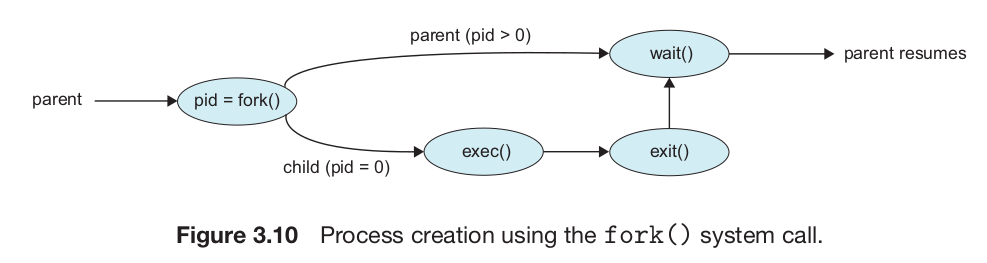
\includegraphics[width=0.9\textwidth]{imagenes/process_creation.png}
	\end{center}

\subsubsection{Terminación}
Un proceso termina cuando ejecuta su última instrucción y pide al sistema operativo que lo borre usando la syscall \texttt{exit()}. En este momento, el proceso envía el código de estado con el que terminó a su padre y el sistema operativo libera todo los recursos que le había asignado.

La terminación puede ocurrir por varios motivos. Un proceso puede causar la terminación de otro usando las syscalls adecuadas (usualmente, esto puede hacerlo solo el proceso padre).

\subsubsection{Un poco más sobre las syscalls mencionadas}
\begin{itemize}
	\item \texttt{pid\_t fork()}: Crea un nuevo proceso. En el caso del creador se retorna el PID del hijo. En el caso del hijo, retorna 0.
	\item \texttt{int\ execve(const char* filename, char* const argv[], char* const envp[] )}: \\ Sustituye la imagen de memoria del programa por la del programa ubicado en filename.
	\item \texttt{pid\_t forkv()}: Crea un hijo sin copiar la memoria del padre, el hijo tiene que hacer \texttt{exec}.

	Un proceso creado con esta syscall comienza con sus páginas de memoria apuntando a las mismas que las de su padre. Recién cuando alguno escriba en memoria, se hace la copia. Esto se llama \textbf{Copy-On-Write}.

	\item \texttt{pid\_t wait(int* status)}: Bloquea al padre hasta que algún hijo termine o hasta que alcance el status indicado.
	\item \texttt{pid\_t waitpid(pid\_t pid, int* status)}: Igual al anterior pero espera a que el hijo con PID \texttt{pid} llegue a ese status.
	\item \texttt{void exit(int status)}: Finaliza el proceso actual.
	\item \texttt{clone(...)}: Crea un nuevo proceso. El hijo comparte parte del contexto con el padre. Es usado en la implementación de threads.
\end{itemize}

\paragraph{Fork Bomb:} Un proceso crea infinitos hijos.
\subsection{Estados de un proceso}\label{procesos::estados}
Durante su ejecución, un proceso va modificando su estado acorde al siguiente diagrama:

\begin{center}
	\vspace*{0.5cm}
	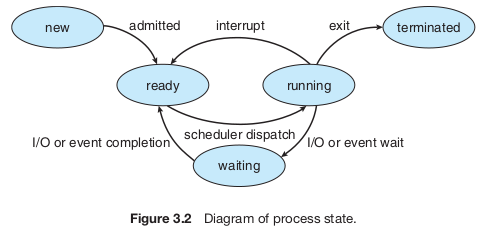
\includegraphics[width=0.9\textwidth]{imagenes/estados-proceso.png}
\end{center}

\begin{itemize}
	\item \textbf{Nuevo (New):} El proceso se está creando.
	\item \textbf{Listo (Ready):} El proceso está listo para ser ejecutado.
	\item \textbf{Bloqueado (Waiting):} El proceso está esperando a que ocurra algo (por ejemplo a que se complete una operación de entrada salida)
	\item \textbf{Ejecutando (Running):} El proceso se está ejecutando.
	\item \textbf{Terminado (Terminated):} El procesó termino de ejecutarse.
\end{itemize}

Es importante notar que solo un proceso puede estar \textbf{ejecutando} en un instante de tiempo de dado. Sin embargo, muchos procesos pueden estar bloqueados o listos simultáneamente.

\subsection{Process Control Block (PCB)}\label{process::pcb}
Cada proceso está representado, en el sistema operativo, por un Process Control Block o Task Control Block. El mismo contiene información asociada a cada proceso, entre ellas:
\begin{itemize}
	\item El estado del proceso
	\item El program counter (la dirección de memoría de la próxima instrucción a ser ejecutada)
	\item Los registros del CPU,
	\item Información de Scheduling, como puede ser prioridad de ejecución
	\item Información de manejo de memoria, como las direcciones de los directorios de paginas o las tablas de segmentación.
	\item Estadísticas de uso del sistema
	\item Información de E/S (que dispositivos está usando, lista de archivos abiertos, etc)
\end{itemize}

\subsection{Scheduler}
\paragraph{Multiprocesador:} Un equipo con más de un procesador.
\paragraph{Multiprogramación:} La capacidad de un SO de tener varios procesos en ejecución.
\paragraph{Multiprocesamiento:} Se refiere al tipo de procesamiento que sucede en los multiprocesadores.
\paragraph{Multitarea:} Es una forma especial de multiprogramación, donde la conmutación entre procesos se hace de manera tan rápida que da la sensación de que varios programas están corriendo en simultáneo.
\paragraph{Multithreaded:} Son procesos en los cuales hay varios \textit{mini procesos} corriendo en paralelo (de manera real o ficticia).

\subsubsection{Context Switching}
Una interrupción hace que el sistema operativo cambie la tarea de una CPU y corra un rutina del kernel. Cuando esto ocurre, el sistema, debe guardar el \textbf{contexto} del proceso que se está ejecutando para poder retornar a la ejecución del mismo cuando termine de atenderla. Este contexto es el PCB del proceso.

\vspace*{0.5cm}
\begin{center}
	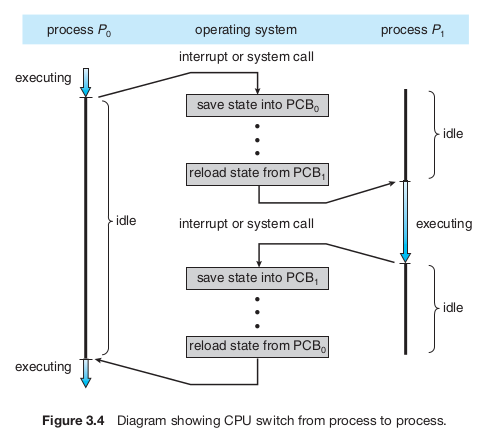
\includegraphics[width=0.625\textwidth]{imagenes/context-switch.png}

\end{center}

	\subsubsection{Colas de procesos}
Una de las características de los sistemas operativos actuales es que nos permiten correr varias aplicaciones a la vez, sin embargo solo un proceso puede estar ejecutando en la CPU. Para darnos la sensación de simultaneidad, el SO hace lo que se llama \textbf{preemption}.

\paragraph{Preemption:} A cada proceso le asigna un \textbf{quantum} o una cantidad de tiempo durante la cual es ejecutado. Una vez que transcurrido ese tiempo, se guarda el contexto del proceso en memoria y se carga el contexto del próximo proceso a ejecutar.

El objetivo de la multiprogramación es intercambiar las tareas que se ejecutan en la CPU lo suficientemente rápido como para que el usuario pueda interactuar con dada programa como si estuviesen ejecutándose simultáneamente.Para esto existe un proceso especial llamado \textbf{Scheduler} que selecciona el próximo proceso que debe ser ejecutado.

El mismo dispone de varias colas de procesos en los que se encuentran los PCB de los procesos en ejecución. Los PCB se van encolando y desencolando de cada cola dependiendo del estado de cada proceso.

\vspace*{0.5cm}
\begin{center}
	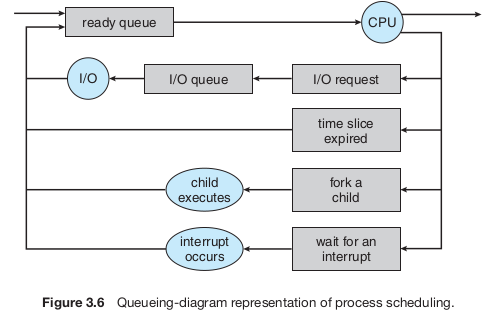
\includegraphics[width=0.8\textwidth]{imagenes/process_queues.png}
\end{center}

\subsection{Inter Process Communication (IPC)}
Los procesos que se están ejecutando concurrentemente en el sistema operativa pueden ser \textbf{procesos independientes} o \textbf{cooperativos}.

\paragraph{Procesos independiente:} Es un proceso que no puede afectar o ser afectado por otros procesos ejecuntandose en el sistema operativo.

\paragraph{Procesos cooperativos:} Son procesos que no son independientes (pueden afectar o ser afectados por otros procesos).

Los procesos cooperativos requieres de un mecanismo de comunicación que les permita intercambiar datos e información. Hay dos modelos fundamentales para hacer esto: \textbf{memoria compartida} y \textbf{Pasaje de mensajes}.

En el modelo de memoria compartida, se establece un área de memoría que es compartida entre procesos. Los procesos pueden intercambiar información leyendo y escribiendo en este área.

En el modelo de pasaje de mensajes, la comunicación se realiza a través de mensajes entre los procesos cooperativos.

\subsubsection{Pasaje de mensaje}
Los mensajes proveen a los procesos un mecanismo que permite que los procesos se comuniquen entre si y sincronicen sus acciones. Un sistema que permite el pasaje de mensajes provee al menos dos operaciones:
\begin{center}
	\texttt{send(message)}\hspace*{1cm}\texttt{receive(message)}
\end{center}

Los mensajes pueden tener una longitud fija o variable. La primera opción es más fácil de implementar pero hace que la programación de tareas sea mas tediosa. Los mensajes de longitud variable necesitan un sistema más complejo pero permite más agilidad a la hora de programar tareas.

Si un proceso $P$ y $Q$ se quieren comunicar, entonces debe existir un \textbf{link de comunicación} entre ellos. Para crear este link, se deben tener en cuenta el tipo de comunicación que se desea ofrecer:
\begin{itemize}
	\item \textbf{Direccionamiento}
	\begin{itemize}
		\item \textbf{Conexión directa:} Cada proceso debe explicitar el nombre del proceso destinatario/receptor:
		\begin{itemize}
			\item \texttt{send(P, message)} - Envía un mensaje al proceso $P$
			\item \texttt{receive(Q, message)} - Recibe un mensaje del proceso $Q$
		\end{itemize}

		En este caso, el link de comunicación se establece automáticamente entre cada par de procesos que quiere comunicarse. Y cada proceso sabe la identidad del otro.

		\item \textbf{Comunicación indirecta:} Los mensajes son enviados a buzones (\textbf{mailboxes}) o puertos (\textbf{ports}). Cada buzón tiene un identificador único. Un proceso puede comunicarse con otro a través de varios buzones.
		\begin{itemize}
			\item \texttt{send(A, message)} - Envía un mensaje al buzón $A$
			\item \texttt{receive(A, message)} - Recibe un mensaje del buzón $A$
		\end{itemize}

		En este esquema, un link se establece entre dos procesos solo si comparten un buzón. Además un link puede estar asociado a varios pares de procesos e incluso puede haber varios links entre dos mismos procesos.

	\end{itemize}
	\item \textbf{Sincronización:} El pasaje de mensajes puede ser bloqueante (síncrono) o no bloqueante (asíncrono):
	\begin{itemize}
		\item \textbf{Envío bloqueante:} El proceso que envía un mensaje espera a que el mismo sea recibido por su destinatario.
		\item \textbf{Envío no bloqueante:} El proceso envía el mensaje y sigue su ejecución.
		\item \textbf{Recepción bloqueante:} El proceso se bloquea hasta que recibe un mensaje.
		\item\textbf{Recepción no bloqueante:} El receptor recibe un mensaje válido o null.
	\end{itemize}
	\item \textbf{Buffering}: Los mensajes intercambiados entre procesos deben almacenarse en una cola temporal. Estas colas pueden ser de tres tipo:
	\begin{itemize}
		\item\textbf{Capacidad Cero:} El link no puede tener mensajes en espera. El remitente debe bloquearse hasta que el mensaje sea recibido.
		\item \textbf{Capacidad acotada:} La cola tiene una capacidad finita $n$ por lo que puede haber a lo sumo $n$ en espera. Si la cola no está llena se puede enviar un mensaje, sino el remitente debe bloquearse hasta que se que haya espacio disponible.
		\item \textbf{Capacidad infinita:} El remitente nunca se bloquea.
	\end{itemize}
\end{itemize}

\subsubsection{Sockets}
Los sockets son los extremos de una comunicación que usan dos procesos para comunicarse a través de una red. Cada socket está identificado por una dirección IP y un número de puerto. 	

En general, en este tipo de links, se usa una arquitecutra cliente-servidor: El servidor espera a que un cliente haga un pedido y, una vez que lo recibe, acepta la conexión del socket del cliente para completar la conexión. El número del socket del servidor, en general, va a ser menor o igual a 1024. Estos puerstos son los puertos conocidos (\textit{well known ports}) e implementan distintos protocolos estandarizados.

Cuando el proceso cliente inicia la conexión, la computadora que lo está ejecutando le asigna un puerto arbitrario cuyo número es mayor a 1024.
\subsubsection{Pipes}
Un \textbf{pipe} es un canal que provee una de las formas más simples de comunicación entre dos procesos aunque tienen sus limitaciones. Al implementar un pipe, se debe tener ciertas consideraciones: 
\begin{enumerate}
	\item ¿El pipe permite comunicación bidireccional o unidireccional?
	\item Si es bidireccional, es \textbf{half-duplex} (para mandar información se debe esperar a que el otro extremo del pipe termina de hacerlo) o \textbf{full-duplex} (la información puede viajar de un lado a otro y viceversa simultaneamente).
	\item ¿Debe existir alguna relación entre los procesos que se están comunicando (por ejemplo, padre-hijo)?
	\item ¿Los procesos se van a poder comunicar dentro de una red o tienen que estar en la misma maquina?
\end{enumerate}

\paragraph{Ordinary pipes:} Permiten que dos procesos se comuniquen en modo productor-consumidor: El productor escribe en un extremo del pipe (extremo de escritura) y el consumidor lee desde el otro extremo (extremo de lectura). Estos pipes son unidireccionales. Si se necesita una comunicación bidireccional se debe crear otro pipe que permita mandar datos en la otra dirección.

Este tipo de pipes requieren que los procesos que se comunican tengan una relación padre-hijo y dejan de existir una vez que la comunicación termina.

\paragraph{Named pipes:} Proveen comunicación bidireccional y no necesitan que los procesos estén relacionados. Una vez que es establecido, varios procesos pueden usarlo para comunicarse y continuan existiendo incluso después de que las comunicaciones hayan finalizado.

\subsection{E/S bloqueante / no bloqueante}
	Cuando un proceso necesita escribir o leer información de algún dispositivo necesita realizar operaciones de \textbf{entrada/salida}

	Estas operaciones son muy lentas por lo que quedarse bloqueado es un desperdicio de tiempo.

	\paragraph{Busy Waiting:} El proceso no hace nada pero no libera el CPU. Se gastan ciclos de procesamiento en hacer nada.

	Para evitar esto se utilizan algunas técnicas que permiten al SO seguir ejecutando mientras espera la respuesta de los dispositivos:

	\begin{itemize}
		\item \textbf{Polling}: El proceso libera la CPU pero todavía recibe un quantum cada tanto que desperdicia hasta que la E/S esté terminada.
		\item \textbf{Interrupciones:} Esto permite la multiprogramación. El SO no le otorgá más quantum al proceso hasta que su E/S esté lista. El hardware comunica esto mediante una interrupción que hace que el proceso se despierte.
	\end{itemize}

	\subsection{Manejo básico de un shell Unix}
\subsubsection{File descriptors:}
	En Unix, cada proceso se crea con una tabla que le permite identificar cuales son los archivos que tiene abiertos. Cada índice es un \textbf{file descriptors} que usa el Kernel para saber como leer/escribir datos en los distintos archivos (en Unix, el teclado y la pantalla se modelan como archivos).
	
	Además, cada proceso hereda de su proceso padre tres archivos abiertos que ocupan los file descriptors 0, 1 y 3 y representan la entrada estándar (\textbf{stdin}), la salida estandar (\textbf{stdout}) y el error estandar (\textbf{stderr}), respectivamente.
	
	Linux provee de dos llamadas al sistema que nos permiten leer/escribir a un archivo usando su file descriptor \texttt{fd}:
	
	\begin{center}
		\texttt{ssize\_t read(int fd, void *buf, size\_t count)}

		\texttt{ssize\_t write(int fd, const void *buf, size\_t count);}
	\end{center}
	
Aquí \texttt{buf} es un puntero a donde se almacenan los datos a leer o escribir y \texttt{count} la cantidad de bytes que hay escribir/leer.

\subsubsection{Comandos de consola}
\begin{itemize}
	\item \texttt{echo} escribe lo que le pasemos como parámetro en su \textbf{stdout}.
	\begin{center}
		\texttt{echo ``Esto es un mensaj''}	\end{center}
	\item \texttt{>} Se le indica a la consola que el \textbf{stdout} se redirija a un archivo:
	\begin{center}
		\texttt{echo ``Esto es un mensaje'' > mensaje.txt}
	\end{center}
	\item \texttt{|} Redirige el \textbf{stdout} de un proceso hacia el \textbf{stdin} de otro:
	
	\begin{center}
		\texttt{echo ``Esto es un mensaje'' | wc -c}
	\end{center}

	En este caso, el primer proceso ejecuta el comando \texttt{echo} que imprime en \textbf{stdout} el mensaje \texttt{``Esto es un mensaje''}. El segundo proceso recibe por \textbf{stdin} lo que se escribió en el \textbf{stdout} del proceso que ejecutó \texttt{echo}
\end{itemize}
\printbibliography[keyword=procesos,title=Bibliografía]

\newpage
	
\section{Scheduling} 
	En sistemas con un único procesador, solo se puede correr de a un proceso por vez. Uno de los objetivos de la multiprogramación es que todo el tiempo se esté ejecutando un proceso para maximizar el uso de CPU.
	
	Cada vez que el CPU entra en estado IDLE, el sistema debe seleccionar alguno de los procesos que estén listos para ser ejecutados. El proceso de selección es llevado a cabo por el \textbf{scheduler} usando la que se llama \textbf{cola de ejecución}.
	
	\subsection{Objetivos de la política de scheduling}
	Diferentes algoritmos de schedulling tienen diferentes propiedades y la elección de los mismos depende de las situación particular del sistema. Por lo general, un algoritmo de schedulling busca optimizar alguna combinación de las siguientes propiedades:
	
	\begin{itemize}
		\item \textbf{Eficiencia}: Maximizar la cantidad de tiempo que el CPU esté ocupado.
		\item \textbf{Rendimiento (Throughput)}: Maximizar el número de procesos terminados por unidad de tiempo.
		\item \textbf{Tiempo de ejecución (Turnaround time)}: Minimizar el tiempo total que le toma a un proceso ejecutar completamente (el intervalo de tiempo desde que el proceso se crea hasta que temina, incluye tiempo de esperas en la cola de procesos).
		\item \textbf{Ecuanimidad (Fairness)}: Que Cada proceso reciba una dosis ``justa" de CPU (para alguna definición de justicia).
		\item \textbf{Carga del sistema (Waiting time)}: Minimizar la cantidad de tiempo que un proceso esté en la cola de espera.
		\item \textbf{Tiempo de respuesta (Response time)}: Minimizar el tiempo de respuesta percibido por los usuarios interactivos.
		\item \textbf{Latencia}: Minimizar el tiempo requerido para que un proceso comienze a dar resultados.
		
		\item \textbf{Liberación de recursos:} Hacer que terminen cuanto antes los procesos que tiene reservados más recursos.
	\end{itemize}
	Muchos de estos objetivos son contradictorios. Si los usuarios del sistema son heterogéneos, pueden tener distintos intereses por lo que cada política de scheduling debe buscar maximizar una función objetivo que es una combinación de estas metas tratando de impactar lo menos posible en el resto.
	
	\subsection{Scheduling con y sin desalojo}
	
	El sistema puede tomar decisiones de scheduling en alguna de las siguientes situaciones:
	\begin{enumerate}
		\item Cuando un proceso pasa de estado \textit{Ejecutando} al estado de espera (por ejemplo cuando hace un request de entrada salida)
		\item Cuando pasa de \textit{Ejecutando} a \textit{Listo}
		\item Cuando pasa de \textit{Esperando} a \text{Listo}
		\item Cuando termina.
	\end{enumerate}
	
	\paragraph{Starvation (Bloqueo indefinido)}: Un proceso sufre de starvation cuando está listo para ser ejecutado pero la CPU nunca le asigna clocks de reloj en lo que ejecutar.
	
	\paragraph{Scheduling sin desalojo:} Tambien conocido como \textbf{coperativo} o \textbf{nonpremptive}, se da cuando las decisiones de scheduling solo toman lugar en las situaciones $1$ y $4$, es decir se espera a que el proceso haya terminado o esté inactivo. Tiene como desventaja que si un proceso muy largo toma control del procesador se puede generar un cuello de botella y otros procesos mas cortos tardarían demasiado en ser ejecutados.
	
	\paragraph{Scheduling con desalojo:} Tambien llamado scheduling \textit{apropiativo} o \textit{preempitve}, se vale de la interrupción del clock para decidir si el proceso actual debe seguir ejecutando o le toca a otro. No da garantías de continuidad a los procesos.
	
	Por lo general se usa una combinación de los dos tipos de scheduling para decidir las políticas adecuadas.

	\subsection{Políticas de scheduling}
	\subsubsection{First In/First Out (FIFO)}
	El algoritmo FIFO (también conocido como First Come, First Served) es una de las políticas de scheduling más simples. Los process control block (PCB) se ubican en una cola, el próximo proceso a ejecutar es el que está en la cabeza. Cuando un proceso está listo para ser ejecutado se lo encola al final.
	
	Por un lado, es simple de implementar. Por otro, el tiempo de espera promedio de un proceso es bastante largo y hay que tener en cuenta que es un algoritmo sin delajo. Si llega un proceso que requiera mucho tiempo de CPU, tapona todos los demás, esto se llama \textbf{convoy effect}.
	
	\subsubsection{Shortest Job First (SJF)}
	Este algoritmo asocia cada proceso con su duración y ejecuta primero aquellos que duran menos. Está ideado para sistemas donde predominan los trabajos batch y está orientado a maximizar el throughput.
	
	Si los procesos ejecutados tienen un comportamiento regular, se puede usa el historial de ejecución para predecir los tiempos ejecución de los procesos actuales. Sin embargo, en sistemas con procesos heterogéneos no es posible saber cuanto tiempo de ejecución va a necesitar cada uno por lo que no es posible implementar este algoritmo.
	
	\subsubsection{Round Robin}
	Este algoritmo está especialmente diseñado para sistemas de tiempo compartido (varios procesos deben usar el cpu al mismo tiempo). Se comporta de manera similar al FIFO, solo que se agrega desalojo para permitir al sistema ejecutar otros procesos.
	
	Para esto se define una pequeña unidad de tiempo llamada \textbf{quantum} durante la cual puede correr cada proceso. Si la ráfaga de procesamiento (CPU Burst) de un proceso es mas chico que el quantum, entonces el mismo la liberará y el scheduler eligirá el siguiente proceso a ejecutar.
	
	Si el CPU Burst toma más de un quantum, entonces se enviará una interrupción al sistema. Éste desalojará el proceso, cambiará el contexto y el proceso que se estaba ejecuntando se pondrá al final de la cola de ejecución.
	
	El rendimiento de este tipo de algoritmos depende del tamaño del quantum. Por un lado, si el quantum es demasiado largo, la política de Round Robind termina siendo una FIFO. Por el otro, si el quantum es extremadamente pequeño se pueden producir una gran cantidad de cambios de contexto, por lo que una gran parte del tiempo del CPU sería gastado solo en esto.
	
	En general, se debe elegir el quantum de tal manera que la mayoria de los procesos termine su CPU Burst durante el mismo pero no tan largo como para que sea un FIFO.
	
	\subsubsection{Multiples colas}
	Otra idea, es serparar los procesos en distintas colas de acuerdo a la duración de su CPU Burst. Cada cola tendrá mas prioridad sobre la otra. Si un proceso toma demasiado tiempo, entonces se lo mueve a una cola con una prioridad menor. 
	
	Este esquema, da mayor prioridad a los procesos interactivos y aquellos procesos que estén esperando demasiado tiempo pueden ser movidos a colas de mayor prioridad para evitar starvation.

\printbibliography[keyword=scheduling,title=Bibliografía]

\newpage
\section{Sincronización de procesos (Memoria compartida)}
Normalmente, los sistemas operativos tratan de prevenir que un proceso acceda a la memoria de otro. Sin embargo, si dos o mas procesos deciden remover esta restricción pueden definir una región de memoria mediante la cual podrán intercambiar información. En este caso, los mismos procesos son los responsables de asegurar que no escriben simultáneamente en esta región.

\paragraph{Contención y concurrencia:} Ocurre cuando uno o más procesos tratan de acceder al mismo recurso de manera simultánea. Esto puede causar que algunas secuencias de ejecución terminen con resultados erróneos.

\subsection{Modelo Productor-Consumidor}
Uno de los paradigmas clásicos de procesos cooperativos con este tipo de intercomunicación es el de \textbf{productor-consumidor}. En este esquema, un proceso \textbf{productor} debe producir información que va a ser consumida por un proceso \textbf{consumidor}.

Una posible implementación de este problema, es definir un buffer en una región de memoria compartida entre ambos procesos en la cual el productor pueda encolar elementos mientras que el consumidor los desencola. Ambos procesos deben estar sincronizados de tal manera que el consumidor no trate de desencolar elementos si la cola está vacía.

Se pueden consierar dos tipos de buffers en esta solución:
\begin{itemize}
	\item \textbf{Unbounded buffer} (buffer infinito): No posee límites de espacio. El consumidor tiene que esperar a que el buffer tenga algo y el productro siempre puede agregarle elementos.
	\item \textbf{Bounded buffer} (buffer limitado): Tiene un tamaño fijo. Si está vacío, el consumidor debe esperar a que haya algo. Si está lleno, el productor debe esperar a que se haya consumido por lo menos un elemento antes de agregar otro.
\end{itemize}

Veamos una solución con buffer limitado:

\vspace*{0.25cm}
\begin{center}
		\textbf{Zona de memoria compartida}
	\begin{minted}[tabsize=28]{cpp}
	buffer in[BUFFER_SIZE];
	int cant = 0;
	\end{minted}
\end{center}
\setlength{\columnseprule}{0.4pt}
\noindent\rule{\textwidth}{0.4pt}
\begin{multicols}{2}
	\begin{center}
	\textbf{Proceso productor}

	\begin{minted}[tabsize=2]{cpp}
	while(true){
		while(counter == BUFFER_SIZE) {};
		in.push(item);
		counter++;
	}
	\end{minted}
\columnbreak
\textbf{Proceso consumidor}
	\begin{minted}[tabsize=2]{cpp}
	while(true){
		while(counter == 0) {};
		item = pop(in);
		counter--;
	}
	\end{minted}
	\end{center}
\end{multicols}
\setlength{\columnseprule}{0pt}

\subsubsection{Condiciones de carrera (race conditions)}
En el ejemplo anterior, si bien el código para cada proceso puede parecer correcto, puede haber errores si ambos se ejecutan de manera concurrente. Supongamos que las lineas \mintinline{cpp}{counter++} y \mintinline{cpp}{counter--} tienen la siguiente forma en lenguaje maquina:
\begin{center}
	\begin{minipage}{0.8\textwidth}
\begin{multicols}{2}
	\noindent\mintinline{cpp}{counter++}:
	\begin{minted}{cpp}
		register1 = counter;
		register1 = register+1;
		counter = register1	
	\end{minted}
	
	\noindent\mintinline{cpp}{counter--}:
	\begin{minted}{cpp}
		register2 = counter;
		register2 = register2-1;
		counter = register2;
	\end{minted}
\end{multicols}
\end{minipage}

\end{center}

Supongamos que el valor inicial de \texttt{counter} es 5, el proceso productor agrega un elemento al buffer, el consumidor quita el primer elemento encolado y ambos procesos ejecutan \texttt{counter++} y \texttt{counter--} de manera concurrente, entonces una posible secuencia de ejecución de estas instrucciones podria ser:

%\vspace*{0.5cm}
\begin{center}
\begin{tabularx}{0.8\textwidth}{|L{1.3}|L{1.3}|C{0.4}|}
	\hline 
	\textbf{Productor} & \textbf{Consumidor} & \textbf{\texttt{counter}} \\
	\hline
	& & 5 \\
	\hline
	\texttt{register1 = counter} & & 5 \\
	\hline
	\texttt{register1 = register + 1} &  & 5 \\
	\hline
	 & \texttt{register2 = counter}  & 5 \\
 	\hline
	 &  \texttt{register2 = register - 1} & 5 \\
  	\hline
	 \texttt{counter = register1} &  & 6 \\
   	\hline
	& \texttt{counter = register2} & 4 \\
	\hline
	\end{tabularx}
\end{center}

En este caso, el consumidor comienza a modificar la variable \texttt{counter} antes de que el productor guarde el valor correspondiente en memoria y no se ``entera" que un nuevo elemento fue agregado a la cola (por lo que todavía habría 5 elementos en ella). Entonces se genera una inconsistencia entre el valor de \texttt{counter} y la cantidad elementos en el buffer.

Este tipo de situaciones se llama \textbf{race condition}: Se da cuando varios procesos pueden acceder y modificar la misma variable de manera concurrente y el valor final de ésta depende del orden particular en el que se hayan realizado los accesos a la misma.

\subsection{Secciones críticas}
La idea es que cada proceso que se esté ejecutando en el sistema tenga un segmento de código, llamado \textbf{sección crítica}, que solo se puede ejecutar cuando ningún otro proceso esté en ella. Es decir, no puede haber mas de un proceso ejecutando su sección crítica al mismo tiempo. Para poder implementar esto, por lo general, se divide el código del segmento en tres partes:
\begin{enumerate}
	\item \textbf{Entry section:} En donde el proceso pide permiso para acceder a la sección crítica.
	\item \textbf{Critical section:} La zona crítica per se, en la que se puede manejar la memoria compartida
	\item \textbf{Exit section:} Donde el proceso avisa al sistema que dejó de realizar operaciones críticas.
\end{enumerate}
\begin{figure}
	\centering
	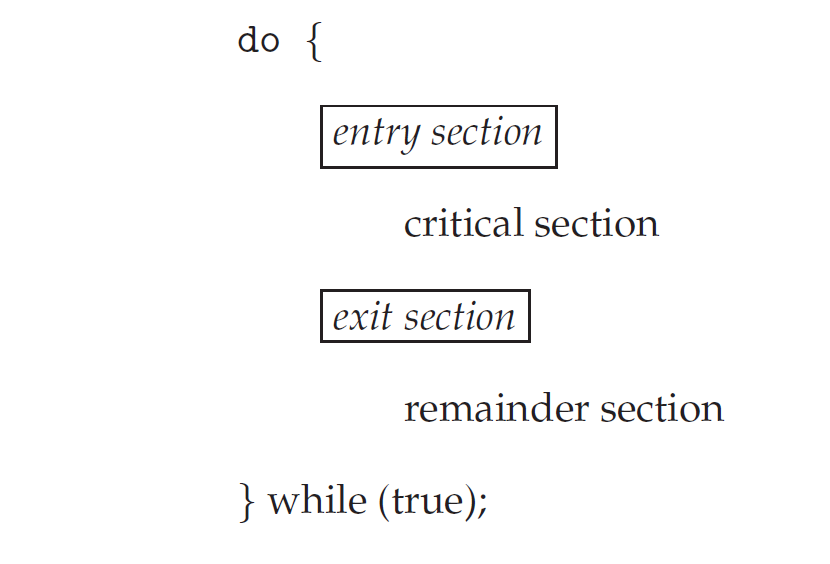
\includegraphics[width=0.5\textwidth]{imagenes/structura-seccion-ciritca}
	\caption{Estructura general de un proceso que implementa sección crítica}
	\label{fig:structura-seccion-ciritca}
\end{figure}

Una buena implementación de esta método debe sastifacer los siguientes requerimientos:
\begin{enumerate}
	\item \textbf{Exclusión mutua}: Si un proceso está ejecutando su sección crítica,
	 entonces ningún otro debe estar ejecutando la suya.
 	\item \textbf{Progreso}: Si un proceso necesita entrar a su sección crítica, entonces se le dará permiso para hacerlo en algún momento.
	\item \textbf{Bounded waiting (espera acotada/no bloqueante	)}: Si un proceso $P$ pide entrar a la sección crítica, entonces hay un límite en la cantidad de veces que se le da mayor prioridad a otros procesos sobre $P$.
\end{enumerate}
\subsubsection{Instrucción TestAndSet}
Los sistemas opertivos modernos proveen una instrucción de hardware especial que nos permite testear y/o modificar una palabra de manera \textbf{atómica}, es decir como unidad no interrumpible de ejecución. Cuando se utiliza, el sistema no ejecuta ninguna otra instrucción hasta que ésta haya terminado. Para abstraernos, de sistemas operativos espécificos, llamemos esta instrucción \texttt{testAndSet()}, la misma toma como paramétro una variable booleana que se va a setear en \mintinline{cpp}{true} y va devolver el valor anterior:

\begin{center}
	\begin{minipage}{0.5\textwidth}
		\begin{minted}[tabsize=2]{cpp}
bool testAndSet(bool* source) {
	bool result = *source;
	*source = true;
	return result;
}
		\end{minted}
	\end{minipage}
\end{center}

En este caso, un sistema de procesos que utilice esta instrucción podría tener una variable booleana compartida llamada \textbf{lock} que controlaria el acceso a la secciónes criticas de cada proceso, si \mintinline{cpp}{lock == false} entonces es posible entrar, si es \mintinline{cpp}{true} el proceso debe esperar:

\begin{minted}[tabsize=2]{cpp}
		bool lock;
		
		void main() {
			while(true) {
				...
				while(testAndSet(&lock)) {};
		
				/* Sección crítica */
		
				lock = false;
				...
			}	
		}
\end{minted}

\subsubsection{Instrucción CompareAndSwap}\label{compareAndSwap}
Es una instrucción primitiva ofrecida por varios porcesadores que toma 3 argumentos: una dirección de memoria, un valor esperado y un valor que se debe escribir en esa posición si se encuentra el valor esperado:

		\begin{minted}[tabsize=2]{cpp}
bool testAndSet(int* value, int expected, int new_value) {
	int temp = *value;
	if(*value == expected) *value = new_value
	return temp;
}
		\end{minted}

\subsubsection{Mutex Lock o SpinLock (busy waiting)} 
La solución basada en hardware presentada en la sección anterior, generalmente es inaccesible a los programadores. Por esta razón, los sistemas operativos diseñan herramientas básicas para implementar secciones críticas: La más simple de ellas es el \textbf{mutex lock}. El mismo contiene de una variable booleana \texttt{avaliable} que indica si el lock está disponible o no y provee dos funciones: 

\begin{itemize}
\item \texttt{acquire()}: Permite a un proceso adquirir el lock y bloquear otros procesos el acceso a su sección crítica. Si un proceso llama a esta función y el lock ya estaba tomado, el proceso queda en espera hasta que el lock se libere.

\begin{minted}[tabsize=2]{cpp}
	void aquire() {
		while(!avaliable) {}; // Busy wait
		avaliable = false;	
	}
\end{minted}
\item \texttt{release()}: Libera el lock para que los procesos bloqueados puedan continuar con su ejecución.
\begin{minted}[tabsize=2]{cpp}
	void release() {
		avaliable = true;	
	}
\end{minted}
\end{itemize}

Ambas funciones deben ejecutarse de manera atómica por lo que generalmente son implementadas usando la instrucción de hardware \texttt{testAndSet()}. La principal desventaja es que requiere de \textbf{busy waiting} (mientras un proceso está en su sección crítica, cualquier proceso que llame a \texttt{aquire()}) debe ciclar continuamente hasta que el lock se libere. Esto es un problema en los sistemas de multiprogramación, donde los ciclos de CPU son compartidos entre varios procesos.

\subsection{Semáforos}
Un semáforo \texttt{S} es una estructura que contiene una variable entera \texttt{value} y una lista \texttt{list} de procesos a las que se puede acceder mediante dos operaciones atómicas:
\begin{itemize}
	\item \texttt{wait()}: Cuando un proceso llama a esta operación, si \texttt{S.value} es negativo entonces debe esperar. Sin embargo, en vez de hacer busy waiting, el proceso se bloquea (entra en estado \texttt{waiting}, ver sección \ref{procesos::estados}) y se encola en \texttt{S.list}. Luego, el control es transferido al scheduler que selecciona otro proceso para ejecutar.
\begin{minted}[tabsize=2]{cpp}
	void wait(S) {
		S.value--;
		if(S.value < 0) {
			agregar este proceso a S.list;
			block();
		}
	}
\end{minted}
	\item \texttt{signal()}: Cuando un proceso termina de ejecutar su sección crítica, llama a esta operación que indica al semáforo que puede despertar alguno de los procesos en espera. Para esto, se quita algun proceso de la lista y se lo pasa a estado \texttt{ready} para que que el scheduler lo vuelva a tener en cuenta.
	\begin{minted}[tabsize=2]{cpp}
		void signal() {
			S.value++
			if(S.value <= 0) {
				quitar proceso P de S.list;
				wakeup(P);
			}	
		}
	\end{minted}
\end{itemize}

Este tipo de semáforos está pensado para administrar la asignación de recursos (de los cuales se tiene una o más instancias) del sistema.

La lista de procesos en espera puede ser implmentada por un campo \texttt{link} en cada process control block (sección \ref{process::pcb}) y la lista de procesos del semáforo en realidad es una lista punteros a PCBs.

%\paragraph{Estructura básica de un proceso con testAndSet()}: Dado un sistema compuesto de $n$ procesos, una posible implementación de secciones críticas que cumplan los tres requirimientos mencionados es la siguiente:
%
%\vspace*{0.25cm}
%\textbf{Zona de memoria compartida}
%	\begin{minted}[tabsize=2]{cpp}
%		buffer waiting[n] = { 0 }; // n = cantidad de procesos
%		bool lock = 0;
%		int  next_process = 0;
%	\end{minted}
%
%\textbf{Proceso número $i$:}
%\begin{minted}[tabsize=2]{cpp}
%		while(true){
%			...	
%			waiting[i] = true;
%
%			while(waiting[i] && testAndSet(&lock)) {}
%			waiting[i] = 0;
%			/* sección crítica */		
%			next_process = next(i);
%			lock = false;
%			...
%		}
%	\end{minted}
%
%Donde \texttt{next(i)} calcula cual es el índice del próximo proceso que debe entrar en la sección crítica de la siguiente forma:
%
%\begin{minted}[tabsize=2]{cpp}
%	int next(int actual_process) {
%		// Buscamos el proximo proceso que este esperando para entrar en 
%		// la sección crítica
%		next = (i + 1) % n;
%		while (next != actual && !waiting[next]) next = (next + 1) % n;
%	
%		// Si no encontré ninguno, entonces no hay nadie esperando 
%		// y libero el lock, sino le doy permiso a que ejecute la sección critica 
%		// al proceso que encontré
%		if(next == actual) lock = false;
%		else waiting[next] = false;
%	}
%\end{minted}

\subsubsection{Monitores y variables de condición}
Aunque los semáforos proveen un mecanismo conveniente y efectivo para realizar la sincronización de proceso, usarlos incorrectamente puede conllevar a errores dificiles de detectar, ya que estos pueden ocurrir en una secuencia de ejecución particular.

Para resolver estos errores, se dasorrollo un tipo abstracto de dato llamado \textbf{monitor} que contiene un conjunto de operaciones que ya aseguran mutual exclusion. El monitor declara variables locales que definen su estado junto con las funciones que operan esas variables (y son la única forma de accederlas).

\begin{minted}[tabsize=2]{cpp}
Monitor M {
/** Declaración de variables compartidas **/
var x;
var y;
var z;

/** operaciones sobre esas variables **/
function op1(...) { ... }
function op2(...) { ... }
function op3(...) { ... }
function constructor(...) { ... }
}
\end{minted}

La implementación del monitor debe asegurar que nunca hay más de un proceso activo dentro del mismo. De esta forma, el programador no debe preocuparse por los requerimientos de sincronización. Sin embargo, la construcción presentada no alcanza para modelar algunos mecanismos de sincronización, por lo que se agrega los mismos lo que se llama \textbf{variables de condición}.

La únicas operaciones invocadas en una variable de condición son \texttt{signal()} y \texttt{wait()}. \texttt{wait()} suspende el proceso hasta que otro proceso llame al \texttt{signal()}. Si no hay procesos esperando, entonces \texttt{signal()} no tiene efecto. Este tipo de variables se puede implementar con semáforos. 

Supongamos que definimos una variable de condición $c1$ sobre el monitor $M$ y que un proceso $P$ invoca $c1.signal()$. Si existe un proceso $Q$ suspendido asociado a $c1$ entonces $Q$ debería poder ingresar al monitor, sin embargo, $P$ sigue estando dentro del mismo. Tenemos dos posibilidades:

\begin{enumerate}
	\item \textbf{Signal and wait:} $P$ se pausa y espera a que $Q$ salga del monitor o espera a que se cumpla otra condición.
	\item \textbf{Signal and continue:} $Q$ espera a que $P$ deje el monitor o espera a que se cumpla otra condición.
\end{enumerate}

Por un lado, tiene sentido dejar que $P$ siga ejecutandose dentro del monitor. Por otro, si permitimos esto, puede llegar a pasar que para el momento en el que $Q$ sea activado, la condición lógica que estaba esperando deje de valer. En muchos casos, lo que se hace es hacer que la ultima instrucción que se ejecuta dentro del monitor sea un \texttt{signal()}. De esta manera, $P$ deja la sección crítica, puede seguir su ejecución y $Q$ puede entrar en su propia sección.

\subsubsection{Deadlock}
La implementación de semáforos puede resultar en una situación donde dos o más procesos se pueden quedar esperando por un evento que solo puede ser causado por otro proceso en espera.  Cuando esto sucede, se dice que estos procesos están en \textbf{deadlock}.

Decimos que un conjunto de procesos está en estado de deadlock cuando cada proceso del conjunto está esperando por un evento que solo puede causado por otro proceso de ese conjunto.

\paragraph{Ejemplo:} Supongamos que tenemos dos procesos $P_0$ y $P_1$ que hacen uso de los semáforos binarios $S$ y $Q$ y se produce la siguiente secuencia de comandos:

\begin{center}
\begin{tabularx}{0.8\textwidth}{|C{0.5}|C{0.5}|L{2}|}
	\hline 
	\textbf{$P_0$} & \textbf{$P_1$} & Efecto \\
	\hline
	& & Ambos semáforos comienzan habilitados \\
	\hline
	\texttt{wait(S)} & & $P_0$ continua ejecución y reserva $S$\\
	\hline
	 & \texttt{wait(Q)} & $P_1$ continua ejecución y reserva $Q$ \\
	\hline
	\texttt{wait(Q)}  & & $P_0$ se suspende hasta que $P_1$ libere $Q$ \\	
	\hline
	 & \texttt{wait(S)} &  $P_1$ se suspende hasta que $P_0$ libere $S$\\	
	\hline
\end{tabularx}
 \end{center}
Al final de la secuencia, ambos procesos están suspendidos porque uno necesita un recurso que tiene en el otro y el sistema entra en deadlock.

\subsubsection{Condiciones de Coffman}
Un sistema puede entrar en deadlock si se cumplen las siguientes condiciones de manera simultanea:

\begin{enumerate}
	\item\textbf{Mutual exclusion}: Hay al menos un recurso que no puede ser compartido. Es decir, es recurso no puede estar asignado a mas de un proceso al mismo tiempo.
	\item \textbf{Hold and Wait}: Un proceso debe tener asigado al menos un recurso y estar esperando por otro que está asignado a otro proceso.
	\item \textbf{No preemption}: El sistema no implementa un mecanismo que le permita quitarle los recursos a los procesos.
	\item \textbf{Circular wait}: Existe un conjunto de procesos \{$P_0,\dots,P_n$\} tal que $P_i$ espera un recurso que está asignado a $P_{i+1}$ y $P_n$ espera un recurso que está asignado a $P_0$.
\end{enumerate}

\paragraph{Livelock:} Se da cuando dos o más procesos no pueden progresar porque hay otros procesos esperando para conseguir un recurso. En este caso, todos los procesos involucrados esperan para poder obtener el recurso y ninguno lo acepta.

\subsection{Correctitud de sistemas concurrentes}
\subsubsection{Modelo del proceso}

\begin{figure}[H]
	\centering
	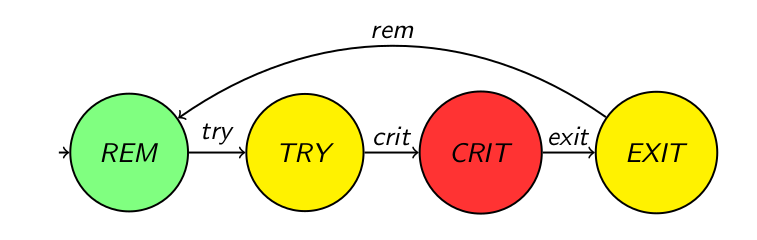
\includegraphics[width=0.7\textwidth]{imagenes/modelo_proceso}
	\caption{Modelo de un proceso según Lynch}
	\label{fig:modeloproceso}
\end{figure}

Un proceso está definido por un aútomata finito con cuatro estados:
\begin{itemize}
	\item \textbf{REM} es el estado en el que se encuentra cuando no está ejecutando en su sección crítica
	\item \textbf{TRY} es el estado en el que se encuentra  cuando está ejecutando los chequeos necesarios para saber si puede entrar en su sección
	\item \textbf{CRIT} es cuando está ejecuntando su sección crítica
	\item \textbf{EXIT} cuando está ejecutando los pasos necesarios para salir correctamente de la sección crítica.
\end{itemize}

\paragraph{Ejecución:} Es una secuencia de estados $\tau = \tau_0 \overset{l_1}{\rightarrow} \tau_1 \overset{l_2}{\rightarrow}\dots$ donde cada $\tau_i$ es un posible estado del sistema y $l_i$ el nombre de la transición utilizada para hacer el pasaje de estados.

%\paragraph{Operadores temporales:} Para hablar de propiedades relacionadas con el tiempo se agregan dos operadores a la lógica clásica. Si $p$ es un predicado lógico, entonces:
%\begin{itemize}
%	\item$\square p$: Siempre vale $p$
%	\item$\diamondsuit p$: En algun momento en el futuro va a valer $p$
%\end{itemize}
\vspace*{.5cm}
Una de las dificultades para demostrar correctitud sobre 
programas concurrentes es que tiene infinitas posibles ejecuciones. Por lo que la noción de \textit{correcto} deja de ser únivoca y pasa a transformarse en comprobar que el sistema cumple ciertas propiedades que en conjunto deben asegurar el comportamiento deseado. Hay tres tipos de propiedades que podemos plantear: 

\begin{itemize}
	\item \textbf{Propiedades de Safety:} Aseguran que no ocurren cosas malas. Son propiedades tales que si no se cumplen entonces existe una ejecución finita del sistema en las que ocurre el evento no deseado. Por ejemplo:
	\begin{itemize}
		\item No hay deadlocks
		\item La función $f$ nunca va devolver null
	\end{itemize}

	\item \textbf{Propiedades de Liveness (Progreso):} Aseguran que, en algún momento, van a ocurrir cosas buenas. Por ejemplo:
	\begin{itemize}
		\item Si se presiona el botón de stop, el tren frena.
		\item Cada vez que el sistema recibe un estímulo, el sistema responde en $X$ tiempo.
	\end{itemize}
	\item \textbf{Propiedades de Fairness:} Los procesos ejecutandose en el sistema reciben su turno con infinita frecuencia. Es decir, los procesos que componen el sistema se ejecuntan regularmente y no son postergados para siempre.
	
	En general, se asume que el sistema estudiado cumple este tipo de propiedades para poder demostrar las propiedades de liveness.
\end{itemize}

\subsubsection{Formalización de algunas propiedades}\label{sincro::form}

\paragraph{Fairness:} Para toda ejecución $\tau$ y todo proceso $i$, si $i$ puede hacer una transición $l_i$ en una cantidad infinita de estados de $\tau$ entonces existe un $k$ tal que $\tau(i)\overset{l_i}{\rightarrow}\tau_{k+1}$. Es decir, que si un proceso puede pasar de un estado a otro, entonces en algún momento lo va a hacer.

\paragraph{Exlusión mutua:} Para toda ejecución $\tau$ y estado $\tau_k$, no puede haber más de un proceso $i$ tal que $\tau_k(i) = CRIT$

%$$\text{EXCL} \equiv \#CRIT \leq 1$$

\paragraph{Progreso:} Para toda ejecución $\tau$, si en $\tau_k$ hay un proceso $i$ en $TRY$ y ningún otro proceso se encuentra en $CRIT$ entonces $\exists$ un momento $k' > k$ tal que $\tau_{k'}(i) = CRIT$.

%$$\text{LOCK-FREEDOM} \equiv \square(\#TRY \geq 1 \land \#CRIT = 0 \Rightarrow \diamondsuit~\#CRIT > 0)$$

\paragraph{Progreso global dependiente (deadlock-free):} Para toda ejecución $\tau$, si para todo proceso que esté en estado $CRIT$ en el momento $k$, en algun momento $k'$ pasa a $REM$ entonces, va a valer que todo proceso $i'$ tal que $\tau_{k'}(i) = TRY$ va entrar en su sección crítica en algun momento $k'' > k'$.

%\begin{itemize}
%\item IN(i) $\equiv i \in TRY \Rightarrow \diamondsuit ~i\in CRIT$
%\item OUT(i) $\equiv i \in CRIT \Rightarrow \diamondsuit~ i\in REM$
%\item STARVATION-FREEDOM $\equiv \forall i.~\square~ OUT(i) \Rightarrow \forall j.~\square ~IN(j)$	
%\end{itemize}

\paragraph{Progreso global absoluto (WAIT-FREEDOM):} Para toda ejecución $\tau$, estado $\tau_{k}$ y proceso $i$, si $\tau_{k}(i) = TRY$ entones existe $k' > k$ tal que $\tau_{k'} = CRIT$

%$$\text{WAIT-FREEDOM}\equiv\forall i.~\square~ IN(i)$$
\printbibliography[keyword=sincro,title=Bibliografía]

\newpage
\section{Programación concurrente (no bloqueante)}
Todos los métodos de sincronización vistos hasta ahora son métodos \textbf{bloquantes} porque un delay inesperado en alguno de los threads puede bloquear el progreso de otros threads. Este tipo de delays es común en multiprocesadores en los que suelene ocurrir cache misses, page faults, cambios de contexto, etc.

\subsection{Algoritmos wait-free y lock-free}
\paragraph{Wait-Free Algorithm:} Un método es \textit{wait-free} si garantiza que termina en una cantidad finita de pasos cada vez que es llamado. Si la cantidad de pasos es acotada, entonces se lo llama \textit{bounded wait-free}. Este tipo de algoritmos aseguran la condición de progreso no bloqueante (el delay en un thread, no neceseriamente bloquea la ejecución de otros threads.)

\paragraph{Population-oblivious Algorithm:} Un algoritmo \textit{wait-free} cuyo rendimiento no depende de la cantidad de threads activos.

\paragraph{Wait-Free Object:} Un objeto tal que todos sus métodos son \textit{wait-free}

\paragraph{Lock-Free Algorithms:} Algoritmos que garantizan que, infinitamente amenudo, alguna llamada a un método termina en un número finito de pasos. 

Esta condición es más débil que la condición de \textit{wait-free}, por lo que cualquier algoritmo \textit{wait-free} es un algoritmo \textit{lock-free} pero no vale la vice versa. Los últimos admiten la posibilidad de que algunos threads sufran de inanición.

\paragraph{Obstruction-Free Algorithm:} Son métodos que terminan en una cantidad finita de pasos si se ejecutan de manera aislada. Este tipo de métodos, obliga a pausar todos los threads que comparten el objeto/región de memoria que va a ser modificado.

\vspace*{0.5cm}
Todos los tipos de algoritmos mencionados en esta sección anterior garantizan que la computación realiza progreso como un todo, independiente de como el sistema maneja los threads.

\subsection{Problema ABA}
Supongamos que tenemos tres threads ($A$, $B$ y $C$) que operan sobre una cola implementada con algoritmos \textit{wait-free}. Y se produce la siguiente situación:

\begin{figure}[H]
	\centering
	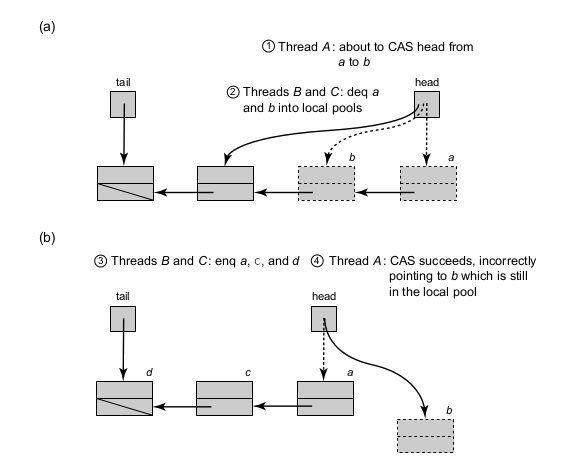
\includegraphics[width=0.7\textwidth]{imagenes/aba-problem}
	\caption{Problema ABA}
	\label{fig:aba-problem}
\end{figure}

\begin{enumerate}
	\item El thread $A$ necesita deseconlar el primer elemento de la cola. Lee el valor almacenado en \texttt{head} y  observa que la cabeza es el nodo $a$ y que el siguiente nodo es $b$. Entonces se prepara para hacer la llamada \texttt{compareAndSwap(\&head, a, b)} (ver sección \ref{compareAndSwap}) pero es desalojado.
	\item Los thread $B$ y $C$ desencolan los nodos $a$ y $b$. y vuelven a encolar el nodo $a$, entonces en la cabeza queda el nodo $a$ y $c$ como el nodo siguiente.
	\item El thread $A$ ejecuta la llamada  \texttt{compareAndSwap(\&head, a, b)}. En este caso, $head = a$ por lo que la condición de la instrucción se cumple y $A$ termina remplazando $a$ por $b$. Dejando incosistente la cola.
\end{enumerate}

Este tipo de situaciones se da a menudo en algoritmos que usan memoria dinámica y operaciones de sincronización  condicionales. Usualmente, una referencia que está por ser modificada por \texttt{compareAndSwap} cambia de $a$ a $b$ y vuelve a ser $a$ por lo que la instrucción termina exitosamente a pesar que la estructura cambió y ya no tiene el efecto deseado.

Una forma facil de resolver este problema es agregar a cada referencia atómica una estampa única que permite definir si el valor fue cambiado o no en el intervalo de tiempo entre que se llamó a la función y efectivamente se ejecuta.

\printbibliography[keyword=progConcurr,title=Bibliografía]


\newpage
\part{Administración de memoria}
\section{Espacio de direcciones}
La parte del sistema operativo que maneja la jerarquía de memoria se llama \textbf{Memory Managment Unit (MMU)}. Su trabajo es mantener un registro de las partes de la memoria que están en uso, reservarla para los procesos que la necesitan y liberarla cuando ya no.

Uno de los métodos más simple de manejo memoria es permitir al programador usar la memoria física directamente.En este caso, se le presenta con un conjunto de direcciones que van desde 0 hasta algún máximo y el proceso ocupa toda la memoria disponible al momento de ejecutarse por lo que se debe esperar a que finalice antes de ejecutar otro.

En sistemas multi-usuarios, n tener varios procesos ejecutando de manera simultanea. Dado que esta situación es difícil de conseguir sin ningún tipo de abstracción, se agregó lo que se conoce como \textbf{espacio de memoria} de un proceso que es el conjunto de direcciones a las que tiene permitido acceder. 

Para separar los espacios de memoria entre distintos procesos, la implementación más simple consiste en agregar dos registros que indiquen cual es la primer dirección de memoria que tiene disponible (\textbf{base register}) y cual es el rango de memoria que puede usar (\textbf{limit register}). 

De esta forma, cuando el programador escribe su programa,  lo hace como si la dirección de memoria más baja disponible fuese la $0000000$. Cuando el proceso haga alguna referencia a memoria, el valor descrito por el programador es sumado al valor del registro base y se comprueba que la dirección resultante no supere el rango definido por el límite.

\subsection{Swapping}
Los métodos vistos hasta ahora permiten asignar a cada proceso un área de memoria. Si queremos ejecutar uno nuevo pero la misma está llena, debemos esperar a que uno o más procesos terminen hasta que se libere el espacio necesario para almacenar el nuevo proceso.

La técnica de \textbf{swapping} trata de resolver este problema guardando los estados de los procesos en ejecución en disco para luego poder cargar el estado de un nuevo proceso y ejecutarlo. Entonces, mientras haya espacio, se cargan y ejecutan como veníamos haciendo hasta ahora. Cuando se llena, se toma alguno de los procesos que se estén ejecutando, se guarda su estado en disco y se lo remplaza por el nuevo. A partir de aquí, cada proceso ejecuta por un tiempo determinado y luego se lo remplaza por otro que esté en la lista de espera.

En este caso no se asegura que los procesos sean cargados en el mismo área de memoria. Cada vez que se recarga uno, se deben reubicar las direcciones a las que hace referencia. 

Además, como no todos los procesos ocupan el mismo espacio en memoria, cuando se realiza un \textit{swap} pueden quedar bloques de memoria vacíos entre dos de ellos. Este efecto se llama \textbf{fragmentación externa} y es un problema porque tras varios swaps pueden quedar varios bloques pequeños vacíos dispersos por toda la memoria. Estos bloques son inutilizables pero si estuviesen todos aglomerados en algún sector específico podrían usarse para correr otro proceso por lo que estaríamos desperdiciando memoria.

Una forma de solucionar este problema es \textbf{compactar la memoria} cada vez que se realiza un swap. Esto es, mover todo los procesos cargados al principio de la memoria, dejando todo el espacio libre al final. Sin embargo, realizar esto cada vez que se realiza un intercambio es demasiado costoso por lo que no es una técnica utilizada.

Por otro lado, si el sistema operativo ofrece la posibilidad de reservar memoria de manera dinámica entonces el área de datos de un proceso debe tener la posibilidad de crecer:
\begin{itemize}
	\item Si la ubicación del mismo es adyacente a un bloque vacío entonces se puede agrandar su área de memoria sin problemas.
	\item Si no es adyante a ningún bloque, entonces el proceso se tiene que mover a un bloque lo suficientemente grande para alojarlo y, si este bloque no existe, se deberá swappear uno o más procesos para crear dicho bloque.
\end{itemize}

\subsection{Manejo de memoria libre}

Cuando la memoria es asignada de manera dinámica, el sistema operativo de mantener un registro preciso de que partes están ocupadas y cuales no. En general, para realizar esto, se puede utilizar alguna de las siguientes estructuras: un \textbf{bitmap} o una \textbf{lista enlazada}.

\begin{figure}[h]
	\centering
	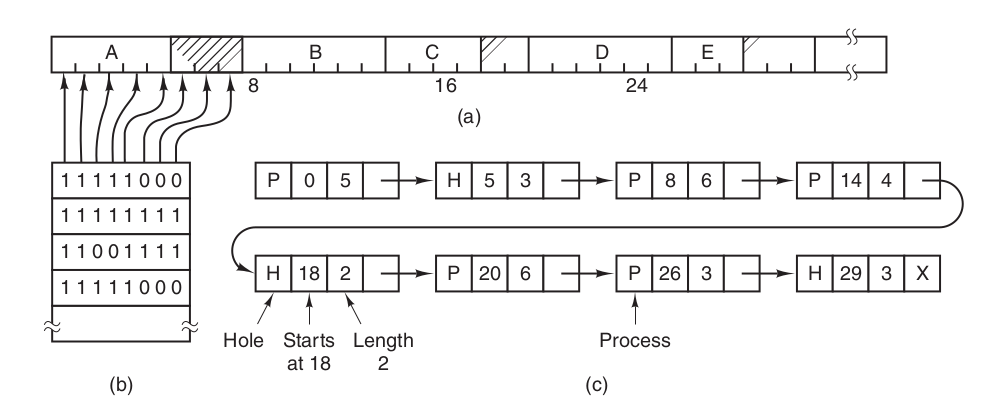
\includegraphics[width=0.65\textwidth
]{imagenes/bitmap-enlazada}
	\caption[Pedazo de memoria con cinco procesos y 3 bloques vacios.]{(a) Pedazo de memoria con cinco procesos y 3 bloques vacios. (b) Bitmap que representa el estado de la memoria. (c) Lista enlazada que representa el mismo estado.}
	\label{fig:bitmap-enlazada}
\end{figure}


\subsubsection{Bitmaps} 
La memoria se divide en bloques de igual tamaño llamados \textbf{unidades de reserva } a las que se les asigna un bit en un array que tiene tantos elementos como bloques haya. Si el bit correspondiente a una unidad se encuentra en cero (0) entonces está libre. Si es uno (1), la unidad está asignada a un proceso.

El tamaño de la unidad de reserva es una decisión de diseño. Mientras más chico sea, más unidades de reservas habrá pero el bitmap se hará más grande. En cambio, si se elige una tamaños demasiado grande, el bitmap se hará más pequeño pero podría desperdiciarse mucha memoria si los tamaños de los procesos no son múltiplos de ese tamaño (muchas unidades reservadas no serán usadas en su totalidad).

El principal problema que tiene esta estructura es que cuando se debe cargar un proceso de $k$ unidades de tamaño, el Memory Managment Unit debe buscar de manera lineal una secuencia de $k$ ceros consecutivos, lo que puede llegar a ser muy lento.

\subsubsection{Listas enlazadas} Otra forma de representar la memoria es mantener una lista enlazada de bloques reservados y espacios libres. Cada entrada de la lista especifica si el bloque pertenece a algún proceso o si está vacío, la dirección de memoria en la que empieza, su longitud y un puntero al próximo bloque. De esta forma es facil encontrar el bloque correspondiente a cada proceso (podemos agregar un puntero en el PCB que apunte al mismo) y liberar su memoria (y combinar bloques vacios) solo implica modificar un par de valores.

\begin{figure}[h]
	\centering
	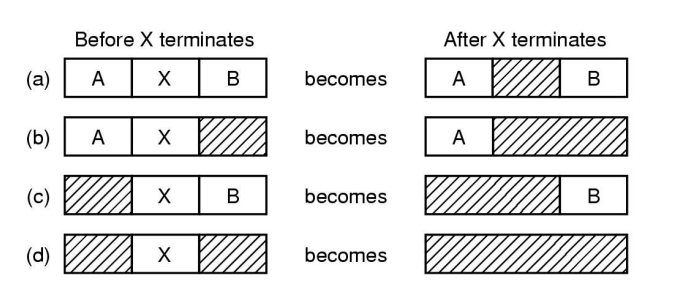
\includegraphics[width=0.7\textwidth]{imagenes/terminacion-proc-memoria}
	\caption{Cuatro combinaciones de vecinos para el proceso X}
	\label{fig:terminacion-proc-memoria}
\end{figure}

\subsubsection{Algortimos para reservar memoria}
Dado un proceso de tamaño $K$ debemos asignarle un espacio de la memoria para que pueda ser ejecutado. Sabemos que el área asignada tiene ser lo suficientemente grande como almacenarlo, el problema es decidir cuál de todos los espacios válidos elegimos. Para esto contamos con los siguientes algoritmos, entre otros:

\begin{itemize}
	\item \textbf{First Fit:} El MMU escanea la meoria hasta que encuentra un bloque lo suficientemente grande como para almacenar el proceso y ocupa la parte necesaria dejando la parte sobrante como un nuevo bloque vacío más pequeño.
	\item \textbf{Best Fit:} El MMU escanea toda la lista (de principio a fin) en busca de todos los bloques en los que podría caber el proceso. Luego le asigna el bloque más pequeño encontrado. En vez de partir un bloque grande, trata de que el bloque extra resultante sea lo más pequeño posible.
	
	Este algoritmo es un poco más lento que el anterior pero tampoco soluciona el problema de fragmentación.
	
	\item\textbf{Quick Fit:} Es una variación de los algoritmos anterior en la que se mantiene una lista de los bloques disponibles ordenado por tamaño. Aquí es facil encontrar un bloque adecuado pero cuando proceso termina o se swappea es más complejo combinar bloques vacíos.
\end{itemize}

\printbibliography[keyword=swapping,title=Bibliografía]

\newpage
\section{Memoria virtual}
Si bien los registros de base y límite nos permiten abstraernos un poco de la memoria, tienen sus limitaciones: Debemos cargar el proceso completo en memoria para poder ejecutarlo. Con los tamaños del softare de hoy en dia, surge la necesidad  de correr programas que no entran en memoria o que si bien entran de manera aislada cuando se lo corre en un sistema multi-usuario con otros procesos, no entran completamente en memoria.

El método diseñado para resolver el problema se conoce como \textbf{memoria virtual}. La idea es que cada proceso tiene definido un espacio de direcciones contiguo a los que puede hacer referencia. Cada una de estas direcciones está mapeada a una dirección física pero dos direcciones virtuales y deben ser traducidas para poder acceder a la información que se está solicitando.

\begin{figure}[h]
	\centering
	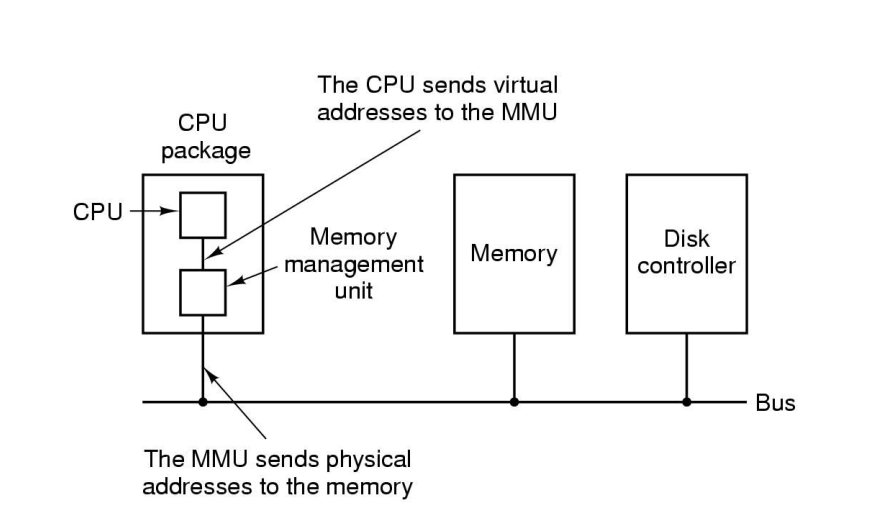
\includegraphics[width=0.7\textwidth]{imagenes/mmu-paging}
	\caption{Funcionamiento del Memory Managment Unit}
	\label{fig:mmu-paging}
\end{figure}

\subsection{Paginación}\label{paginacion}
La mayoría de los sistemas que usan memoria virtual implementan una técnica conocida como \textbf{paginación}: Cada programa tiene asignado un espacio de memoria virtual dividido en pedazos llamados \textbf{páginas}. Cada página es un rango continuo de direcciones y está mapeada a un pedazo de memoría física llamado \textbf{page frame}.

\begin{figure}[h]
	\centering
	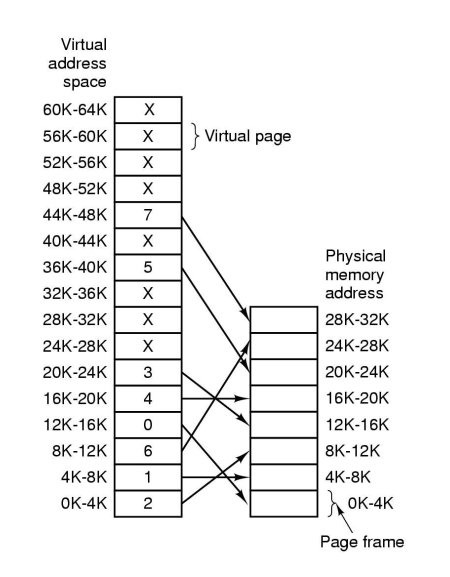
\includegraphics[width=0.6\textwidth]{imagenes/paging-mapping}
	\caption{Ejemplo de mapeo de direcciones virtuales a direcciones físicas}
	\label{fig:paging-mapping}
\end{figure}

Entonces un proceso puede comenzar a ejecutar sin necesidad que todas sus páginas estén cargados en memoria. Cuando hace referencia a una \textbf{dirección virtual}, la misma se envía al MMU que se fija si el page frame correspondiente está cargado en memoria. Si lo está entonces recupera la información pedida. Si no, emite un \textbf{page fault} que es atrapado por el sistema operativo que se encarga de traer el page frame necesario para poder continuar con la ejecución.

\subsubsection{Page tables} 
En esta implementación usamos una tabla para mapear direcciones virtuales a físicas. Dada una dirección virtual, la partimos en dos: 
\begin{itemize}
	\item \textbf{Número de página:} Son los bits más significativos. Nos indicara cuál es la posición de la tabla que apunta al page frame que contiene la dirección física deseada.
	\item \textbf{Offset:} Son los bits menos significativos. Se suman a la dirección del page frame encontrado  para poder conseguir la dirección de memoria física deseada.
\end{itemize}

\begin{figure}[h]
	\centering
	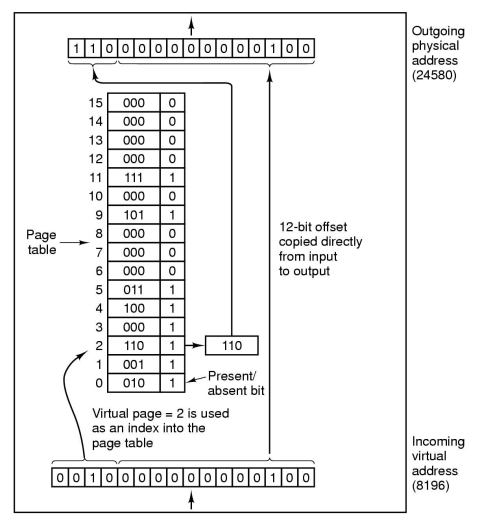
\includegraphics[width=0.5\textwidth]{imagenes/virtual-a-fisica}
	\caption[]{Conversión de una dirección virtual a una física}
	\label{fig:virtual-a-fisica}
\end{figure}

\subsubsection{Estructura de una entrada de la tabla de páginas}
Cada entrada de esta tabla tendrá la siguiente información, en la mayoría de los sistemas:

\begin{itemize}
	\item \textbf{Número de page frame:} El page frame al que mapea una página virtual.
	\item \textbf{Bit de presente/ausente:} Este bit es el que usa la MMU para saber si la entrada es válida (el page frame está cargado en memoria) o no.
	\item \textbf{Bit de protección:} Indica que tipo de accesos son permitidos. En su versión más simple, si está activo, el proceso solo puede leer. Si no lo está entonces puede escribir y leer.
	\item \textbf{Bit dirty:} Indica si la página fue modificada o no por el proceso. Este bit lo usa el sistema operativo cuando necesita desalojar el page frame. Si fue modificado, debe copiarse a disco sino la podemos sobrescribir ya que la copia en disco sigue siendo valida.
	\item \textbf{Bit de referencia:} Indica si la página fue referenciada por el proceso (tanto para escribir como para leer). Este bit tambien es usado por el sistema operativo para ayudarlo a decidir que page frame desalojar en caso de ser necesario. Las páginas que no están siendo usadas son mejores candidatos que aquellas que fueron referenciadas últimamente.
\end{itemize}

\subsection{Optimizaciones para paging}
Un sitema con paginación tiene que tener en cuenta dos cosas:
\begin{itemize}
	\item El mapeo de direcciones virtuales a físicas debe ser rápido.
	\item Si el espacio virtual es grande, entonces la tabla de páginas tambien lo será.
\end{itemize}
\subsubsection{Translation Lookaside Buffer (TLB)}
Para acelerar el mapeo de direcciones, se agregó al procesador una caché llamada \textbf{Translation Lookaside Buffer} o \textbf{Memoria asociativa} que permite realizar el mapeo sin tener que acceder a la tabla de páginas.

Cada entrada de esta cache contiene información sobre una página (su índice en la tabla de páginas, bit de protección, dirty y el page frame que le corresponde) además de un bit que indica si la entrada es válida.

Cuando la MMU recibe una dirección virtual, el hardware primero se fija si el número de página está presente en la TLB comparandolo simultáneamente con todas las entradas de la misma. Si lo encuetnra y el acceso no viola los bits de protección entonces el page frame se obtiene directamente. Si lo encuentra pero el proceso no tiene los permisos necesarios, entonces se genera un page fault.

Cuando ninguna de las entradas contiene el número de página buscado, el MMU detecta el \textit{miss} y realiza la búsqueda en la tabla de páginas de manera normal. Una vez encontrada, borra una de las entradas de la TLB y la remplaza con la entrada de la página encontrada.

Cuando una entrada se borra de la TLB, el bit de dirty se copia a la entrada de la page table correspondiente.

\subsubsection{Multilevel Page Tables}
El segundo problema que teniamos que resolver era como manejar tablas de páginas muy grandes. Esto se hace usando \textbf{tablas de página multinivel}. 

La idea es evitar que la tabla de páginas se mantenga completamente en memoria. En particular, aquellas entradas que no se necesitan no deberían mantenerse cargadas. Para conseguir esto, creamos un \textbf{directorio de páginas} y particionamos la tabla de páginas en partes iguales.

\begin{figure}[h]
	\centering
	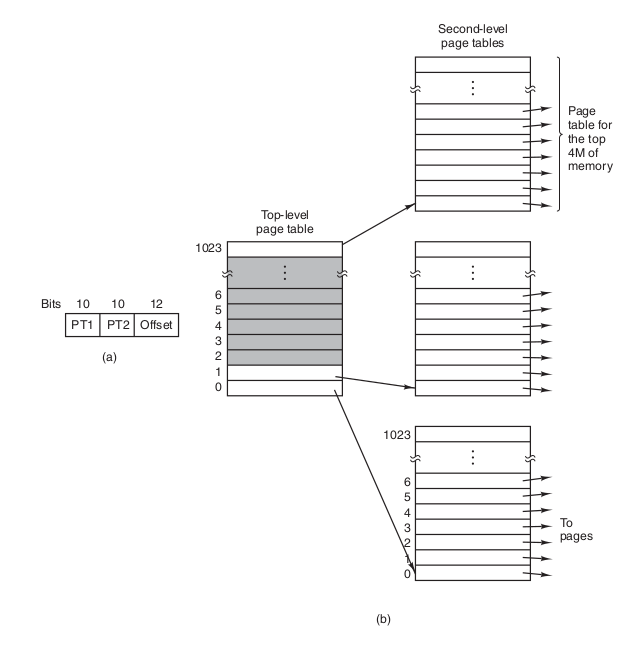
\includegraphics[width=0.5\textwidth]{imagenes/multilevel-page-table}
	\caption{Descomposición de una dirección virtual en paginación multinivel}
	\label{fig:multilevel-page-table}
\end{figure}

El directorio de páginas contiene información sobre como ubicar la tabla de páginas que necesitamos para mapear la dirección virtual. De esta forma, cuando la MMU recibe un dirección virtual, la divide en tres partes:

\begin{itemize}
	\item Los primeros bits son usados como índice para ubicar la entrada en el directorio de páginas que nos permite conseguir la tabla correspondiente a esa dirección.
	\item La segunda parte se usa como número de página dentro de esa tabla para encontrar el page frame deseado.
	\item Y la última parte es el offset dentro del page frame encontrado.
\end{itemize}

La entrada del directorio de páginas es igual que la de una tabla de páginas normal. Si el bit de presente no está activado cuando buscamos una tabla determinada, se genera un page faul y el sistema operativo debe cargar en memoria la tabla correspondiente.

\subsection{Algoritmos de reemplazo de páginas}
El mejor algoritmo de remplazo de páginas es imposible de implementar: Remplazar la página que menos se va a utilizar en el futuro.

\subsubsection{Not Recently Used (NRU)}
Como dijimos, las entradas de las tablas de páginas tienen dos bits (bit dirty y referenced) que nos dan información sobre como se estuvo usando cada una de ellas. Gracias a ellos, se pueden crear algoritmos de paginación con distintos criterios que nos permitan saber como remplazar page frames a medida que se van ejecutando los procesos.

Cuando un proceso comienza su ejecución, ambos bits están desactivados para todas las entradas de la tabla. Además, el bit de referencia se desactiva periódicamente para distinguir las entradas que fueron accedidas recientemente de aquellas que no.

Cuando ocurre un page fault, el sistema operativo inspecciona todas las páginas y las divide en 4 categorías:

\begin{itemize}
	\item Clase 0: No referenciadas, no modificadas
	\item Clase 1: No referenciadas, modificadas
	\item Clase 2: Referenciadas, no modificadas
	\item Clase 3: Referenciadas y modificadas
\end{itemize}

El algoritmo NRU remueve una página random de la clase más baja no vacía. En este algoritmo está implicita la ideae de que es mejor swapear una página modificad que hace rato que no se referencia, a una página no modificada que se está usando.

\subsubsection{First In, Firt Out (FIFO)}
El sistema operativo mantiene una lista de todas las páginas cargadas en memoria. La última página de esta lista es la ultima que fue cargada y la primer es la que más tiempo estuvo en memoria.

Cuando se realiza un page faul, se remueve el primer elemento y se encola la nueva página.

\paragraph{Second Chance Algorithm:} Se modifica el FIFO para que se inspecciones el bit de referencia de la página más vieja. Si el bit está en cero, entonces la página es vieja y no está en uso por lo que es remplazada. 

Si el bit está seteado, entonces el bit se limpia y la página se encola al final de la lista. Luego, la búsqueda continua. Si todas las páginas fueron referenciadas, entonces, se revisan todas las páginas cargadas hasta volver a empezar y se termina eliminando la que había sido la primer página analizada.

\subsubsection{Least Recently Used}
Una buena aproximación al algoritmo optimo se basa en la observación que las páginas que han sido más usadas en las últimas instrucciones probablemente vuelvan a ser usadas. En cambio, las páginas que no son usadas hace rato probablemente sigan sin usarse.

En este algoritmo, cuando sucede un page fault, se descarga la página que no ha sido usada durante el mayor rango de tiempo.

\subsubsection{Working Set}
En su forma más pura, los procesos comienzan sin ninguna de páginas en memoria. Tan pronto como el CPU trata de conseguir la primer instrucción se produce un page fault, causando que el sistema operativo traiga la página que contiene la primer instrucción. Por lo general, se producen varios page fault para traer memoria variables globales y el stack. 

Después de un tiempo, el proceso tiene la mayoría de las páginas que necesita para poder ejecutar con relativamente pocos page fault. Esta estrategia se llama \textbf{demand paging} porque ninguna página se carga a no ser que sea necesaria.

La mayoría de los procesos exhiben \textbf{localidad de referencia}, esto significa que durante cualquier etapa de ejecución el proceso referencia solo una pequeña fracción de sus páginas disponible. 

El conjunto de páginas que un proceso está usando se llama conjunto de trabajo (\textbf{working set}). Si este conjunto entra complentamente en memoria, entonces el proceso podrá correr realizando poco page faults. Si la memoria disponible no alcanza para almacenarlo entonces el proceso generara page faults constantemente y se alentizará su ejecución. Este efecto se llama \textbf{trashing}.

Por esta razón, muchos sistemas tratan hacer un seguimiento del working set de cada proceso y asegurarse que esté completamente en memoria antes de dejar que se ejecute. Este método se llama \textbf{working set model} y está diseñado para disminuir el ratio de page faults provocados por proceso. Cargar páginas antes de que los procesos la necesiten es una técnica llamada \textbf{prepaging}

\subsection{Page fault}
Estos son los pasos que realiza un sistema opertivo una vez que el MMU emite un page fault:

\begin{enumerate}
	\item El hardware emite el page fault que es atrapado por el sistema operativo.
	\item Se guarda el program counter de la instrucción fallida y el estado del proceso.
	\item El sistema operativo se fija cual es la página que necesita el proceso. 
	\item El sistema operativo controla que la dirección pedida sea válida y que la protección de la misma sea consistente con el acceso. Si no lo es, se manda una señal al proceso o se lo mata. Si la dirección es válida y no hay un protection fault, el sistema se fija si hay page frames libres. Si no los hay, se usa alguno de los algoritmos de remplazo de páginas.
	\item Si el page frame a desalojar está modificado, la página se marca para transferir a disco. Se realiza un context switch suspendiendo la rutina de interrupción y dejando que otro proceso se ejecute mientras se completa la transferencia.
	\item Una vez completada la transferencia, el sistema operativo, busca la dirección del disco en la que está almacenada la página y la marca para cargarla en memoria. Mientras sucede esta transferencia se vuelve a suspender la rutina y se deja ejecutar a otro proceso.
	\item Despues de que la página está cargada en memoria, se actualizan las tablas de página para reflejar los cambios y la entrada se marca como válida.
	\item El proceso vuelve a entrar en la cola del scheduler y el estado se reseta a como estaba antes de ejecutar la instrucción que generó el page fault.
\end{enumerate}

\printbibliography[keyword=memoriaVirtual, title=Bibliografía]

\newpage
\section{Segmentación}
La memoria virtual discutida hasta ahora es unidimensional: A cada proceso se le asigna un conjunto de direcciones que van desde 0 hasta una dirección máxima. Cuando el compilador genera un proceso divide este espacio en partes de uso espécifico (por ejemplo, stack, tabla de constantes, tabla de símbolos, código fuente, etc). 

Sin embargo, esta division puede llegar a traer problemas. En la figura \ref{fig:organizacion-proceso}, por ejemplo,  la tabla de símbolos se llenó y no puede seguir creciendo porque las próximas direcciones contienen el código del programa.

\begin{figure}[h]
	\centering
	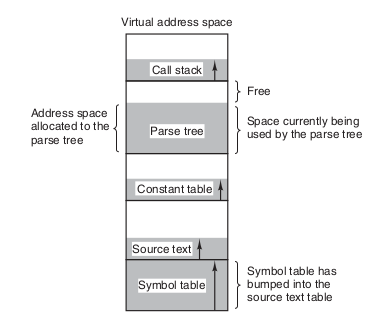
\includegraphics[width=0.7\textwidth]{imagenes/organizacion-proceso-virtual-unidimensional}
	\caption{Organización de un proceso con memoria virtual }
	\label{fig:organizacion-proceso-virtual-unidimensional}
\end{figure}

Una solución a este problema es proveer al proceso de varios espacios de memoria virtuales completamente independientes llamados \textbf{segmentos}. Cada segmentos consiste en una secuencia lineal de direcciones que van desde cero hasta algún valor máximo y como son independiente cada uno puede crecer o contraer sin afectarse entre si.

Para especificar una dirección ubicada en un segmento, el programa debe enviar una dirección que se divide en dos partes: Un número de segmento y la dirección virtual dentro de ese segmento.

Esta técnica además facilita la implementación de librerias compartidas. Dado que cada fragmento es una entidad lógica que el programador sabe que contiene, cada uno de ellos puede tener distinto tipos de protección.

En muchos sitemas es común encontrar la segmentación implementada con paginación para segmento.

\subsection{Shared Libraries}
En sistemas multiprogramables, es comun tener varios usuarios corriendo el mismo programa de manera simultánea. Incluso un único usuario puede estar corriendo varios programas que hagan uso de las mismas rutinas. Cuando esto sucede, los segmentos de código de cada proceso apuntan a la misma tabla de páginas (como el código es solo lectura, ambos procesos pueden accederlas sin problemas).

Sin embargo, hay que tener en cuenta que cuando dos o mas procesos comparten las páginas y uno termina, no debemos desalojar las páginas compartidas ya que cuando se vuelva a ejecutar el otro proceso, se generarian varios page faults hasta que todas las paǵinas desalojadas vuelvan a estar en memoria. Por esta razón, debemos mantener una estructura que nos permita identificar rápidamente cuales son las páginas compartidas para evitar esta situación.

\subsubsection{Copy On Write}
Tambien se puede compartir páginas que contenga datos aunque hay que tener algunas consideraciones más. En los sistemas UNIX, en particular, cuando se realiza una llamada a \texttt{fork()}, el proceso padre comparte todas sus páginas con el proceso hijo pero cada uno tiene su propio conjunto de tablas de páginas. Sin embargo, en ambos procesos se marca a todas las páginas como \textit{Read Only}. 

Mientras ambos procesos solo hagan lecturas, la situación se mantiene. Tan pronto como algunos de los dos necesita realizar una modificación, se genera un protection fault que es interceptado por el sistema operativo. El mismo realiza una copia de la página que se quiere modificar y ahora cada proceso tiene su propia copia de la información con acceso de escritura/lectura. Así, las próximas modificaciones a esa página suceden sin interrupciones. Esto implica que la información que las páginas que no son modificadas nunca no necesitan ser copiadas.

Esta técnica es conocida como \textbf{copy on write}.

\printbibliography[keyword=segmentacion, title=Bibliografía]
 
 

\newpage
\part{Administración de entrada/salida}

\section{Subsistema de I/O}
Los elementos básicos de hardware, como puertos, buses y controladores se conectan una gran variedad de disposivitos de entrada/salida que varian en sus funciones y velocidades por lo que se necesitan varios métodos para controlarlos. Éstos forman parte del \textbf{subsistema de I/O} y son encapsulados en módulos llamados \textbf{drivers}. 

Los drivers presentan una interfaz de acceso uniforme a los subsitemas de entrada/salida, eliminando la necesidad de que el sistema operativo sepa como manejar las particularidades de cada dispositivo. Los mismos corren con máximo privilegio y de ellos depende el rendimiento de todo el subsistema de entrada/salida

La mayoría de los dispositivos que se usan en una computadora pueden ser clasificado como de almacenamiento (discos, memorias flash), de transmissión (conexiones al internet, bluetooth) e interface de usuarios (pantallas, teclados, mouse).

\paragraph{Puerto (Port):} Es un cable mediante el cual se comunican los dispositivos de entrada/salida con el sistema

\paragraph{Bus:} Es un conjunto de cables compartidos por varios dispositivos junto con un protocolo específico que define un conjunto de mensajes que pueden ser enviados a los mismos.

\paragraph{Controlador:} Es un dispositivo que puede operar un puerto, un bus u otros dispositivos. Algunos controladores pueden llegar a tener un pequeño procesador, microcodigo y memoria privada integradas para implementar protocolos complejos. Un ejemplo de esto son los controladores \textbf{Small Computer System Interface (SCSI)} que se encargan de comunicar los discos con el sistema

\begin{figure}[h]
	\centering
	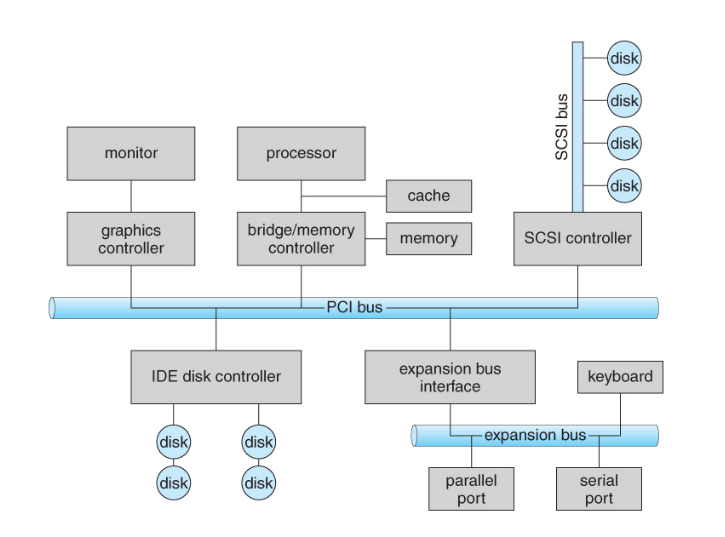
\includegraphics[width=0.5\textwidth]{imagenes/estructura-basica-bus}
	\caption{Estructura típica de un Bus}
	\label{fig:estructura-basica-bus}
\end{figure}

\subsection{Interacción con los dispositivos}
La interacción entre el sistema y un controlador puede tomar varias formas. La más simple es conocida como \textbf{polling} o \textbf{busy-waiting}. Con este método, el sistema está constantemente verificando el estado de un dispositivo hasta que está listo para ser usado. Una vez que el dispositivo está listo, le manda un pedido y vuelve al ciclo de verificación hasta que el dispositivo marca que el pedido fue atendido.

Esté método tiene sentido en dispositivos que deben ser atendidos rápidamente. Por ejemplo,el buffer de los controladores de teclados es muy pequeño y podríamos perder información si el sistema tarda demasiado en leer los bytes del mismo.

Sin embargo es ineficiente cuando el dispositivo se usa poco y hay otros procesos que deben terminarse. En estos casos es más eficiente configurar los controladores para que notifiquen al CPU cuando el dispositivo está listo para atender un pedido. El mecanismo que permite implementar esto es llamado \textbf{interrupciones}.

\subsubsection{Interrupciones}
El CPU tiene un cable llamado linea de pedido de interrupciones (\textbf{interrupt-request line}) que se chequea cada vez que se termina de procesar una instrucción. Cuando se detecta una interrupción en este cable, el sistema determina cuál fue la causa, realiza el procesamiento necesario para atenderla y luego sigue ejecutando los procesos del usuario.

\subsubsection{Direct Memory Access}
Para dispositivos que realizan transferencias de grandes cantidades de datos, como discos rígidos, se usa un procesador especial llamado controlador de acceso directo a memoria (\textbf{Direct Memory Access Controller}).

El sistem debe avisarle al controlador DMA que desea realizar una transferencia y le pasa un puntero a la data que quiere transferir, un puntero a donde quiere hacerlo y la cantidad de bytes que deben ser transferidos. El controlador procede a realizar la transferencia mientras el CPU pasa a otra tareas por lo que no es necesario esperar a que termine la transferencia para seguir trabajando.

\subsection{Drivers}
Podemos abstraer las diferencias especificas entre los dispositivos de entrada/salida clasificandolos de una manera más generalizada. Cada clase es accedida a través de una conjunto estandarizado de funciones (una \textbf{interfaz}) que debe ser implementada por los drivers de cada dispositivo.

Las interfaces presentadas por el sistema deben en tener en cuenta las siguientes características de los dispositivos:

\begin{itemize}
	\item \textbf{Tamaño de transferencia } (character-stream or block-steram): Los dispositivos \textbf{character-stream} transfieren byte a byte, mientras que los dispositivos de transferencia bloques transmiten una unidad de información compuesta de varios bytes.
	\item \textbf{Acceso secuencial o aleatorio}: Un dispositivo secuencial transfiere información en un orden determinado por el dispositivo, mientras que los usuarios de un dispositivo de acceso aleatorio pueden pedir que se busque cualquier porción de la memoria disponible.
	\item \textbf{Sincróno o asincróno:} Un dispositivo síncrono realiza las transferencia con un tiempo de respuesta predecible y coordina con otros aspectos del sistema. Un dispositivo asíncrono exhibe tiempos de respuesta irregulares que no se pueden coordinar con otros eventos del sistema.
	\item \textbf{Compartido o dedicado:} Un dispositivo compartido puede ser usado por varios procesos o thread de manera concurrente, mientras que uno dedicado no. 
	\textbf{Velocidad de operación:} Puede variar de uno pocos bytes por segundo a varios gigabytes por segundo, dependiendo el dispositivo.
	\textbf{Tipo de comunicación:} Puede ser dispositivos de solo escritura, de solo lectura o de escritura/lectura.
\end{itemize}

\subsubsection{Block devices}
La interfaz de los dispositivos de bloque capturan todos los aspectos necesarios para acceder a dispositivos de almacenamiento. Los comandos básicos que se espera que respondan son: \texttt{read()} y \texttt{write()}. Además de la operación \texttt{seek()}si el dispositivo permite acceso aleatorio.

Sin embargo, hay aplicaciones especiales (como los motores de bases datos) que pueden preferir acceder a los dispositivos como si fuesen un arreglo lineal de bloques (\textbf{raw I/O}) debido a que implementan sus propios buffers o técnicas de escrituras. Por estar razón, se permite a esos programas realizar los accesos directos y evitar el comportamiento default del sistema operativo.

\subsection{Spooling}
Su nombre proviene de \textbf{Simultaneous Peripheral Operation On-Line} y consiste en un buffer que almacena información que se debe enviar a un dispositivo, como una impresora, que no puede aceptar información de manera intercalada. Aunque una impresora puede ejecutar un solo trabajo por vez, varias aplicaciones pueden requerir su uso de manera concurrente y es necesario que sus salidas no se mezclen. El sistema operativo resuelve este problema interceptando todos los pedidos y enconlandolos en este buffer. Cuando la impresora está lista para responder un nuevo pedido, el sistema copia el siguiente archivo de la cola.

Hay que tener en cuenta que este proceso es visible a nivel usuario y es manejado por el sistema operativo. El kernel y los controladores actuan de manera normal.
 
\printbibliography[keyword=drivers, title=Bibliografía]

\newpage
\section{Almacenamiento Secundario}
\subsection{Tipos de discos}
\subsubsection{Discos Magnéticos}\label{discosMagneticos}
Son la mayor parte del sistema de memoria secundario en las computadoras modernas. Un disco rígido, consiste en un conjunto de platos (\textbf{platters}) con una forma circular y varios cabezales de lectura-escritura (\textbf{read-write head}) que ``vuelan" sobre su superficie:

\begin{figure}[h]
	\centering
	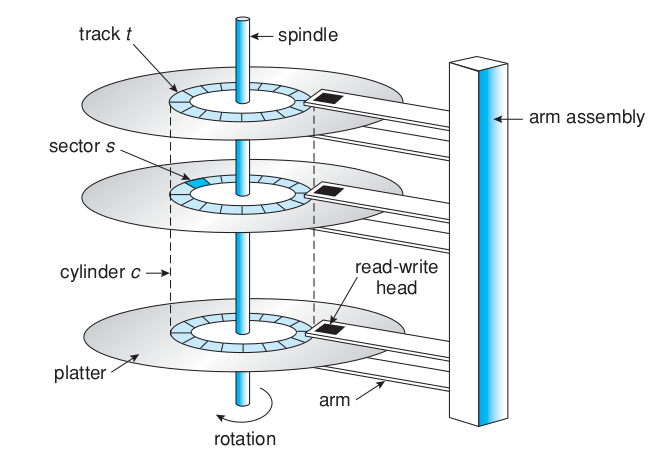
\includegraphics[width=0.7\textwidth]{imagenes/mecanismo-lectura-disco}
	\caption{Mecanismo de lectura/escritura de un disco}
	\label{fig:mecanismo-lectura-disco}
\end{figure}

Todos los cabezales están unidos a un brazo que los mueve de manera unísona. Cuando un disco está en uso, un motor gira sus platos a alta velocidad y el brazo mueve los cabezales de manera radial (desde el centro del plato hasta el perímetro del mismo y viceversa).

La superficie de cada plato está divida en sectores lógicos llamados \textbf{tracks} que están subdivido en \textbf{sectores}. El conjunto de \textbf{tracks} que estan a la misma distancia del brazo se llama \textbf{cilindro}. Cada disco puede tener miles de cilindros y cada track cientos de sectores por lo que en general la capacidad de estos dispositivos se mide en gigabytes.

La velocidad de un disco se divide en dos partes:
\begin{itemize}
	\item \textbf{Velocidad de transferencia (Transference Rate):} La velocidad a la que la infromación viaja entre el disco y la computadora.
	\item \textbf{Tiempo de posicionamiento (random-acces time):} Que es el tiempo que tarda el disco en encontrar un sector determinado. Este tiempo se puede dividir en dos partes:
	\begin{itemize}
		\item \textbf{Tiempo de búsqueda (seek time):} El tiempo necesario para mover el cabezal al cilindro adecuado.
		\item \textbf{Latencia rotacional (Rotational Latency):} El tiempo necesario para que el sector llegue al cabezal ya posicionado
	\end{itemize}
\end{itemize}
Generalmente, los discos pueden transferir varios megabytes de datos por segundo y los tiempos de búsqueda y de giro toman varios milisegundos.

Un disco puede ser removible permitiendo que varios discos se vayan montando y desmontando a medida que sea necesario. Algunas formas de discos removibles incluyen: CDs, DVDs y Blu Rays y memorias \textbf{flash}.

\subsubsection{Discos de estado solido (SSD)}
Un disco de estado sólido es una memoria no volátil que es usada como disco rígido. Tienen las mimas características que los discos clásicos pero son más seguros porque no tienen partes mobiles y son más rápidos por queno tienen latencia y ni tiempo de búsqueda. Además, consumen menos energía. Sin embargo, son más caros que los discos tradicionales, tienen menos capacidad y tiempos de vida más cortos.

Otro problema que tiene este tipo de discos es llamado \textbf{write amplification}, en el cual la cantidad de información escrita en el disco es un múltiplo de la cantidad lógica que se intentó escribir. En las memorias flash, es necesario borrar la memoria antes de poder escribirla pero las operaciones de borrado tienen una granularidad bastante mayor a la de escritura. Entonces, el proceso de escribir a memoria, muchas veces implica mover la sección usada de un bloque a alguna ubicación no usada del disco y luego borrar todo el bloque para luego poder escribir en la ubicación deseada.

Osea que una escritura puede requerir que se lea, actualize y reescriba alguna parte de la memoria ya utilizada en una nueva ubicación. Borrar la ubicación inicial y luego escribir los datos que se desean guardar. Este efecto multiplicador aumenta la cantidad de escrituras necesarias en el disco, lo que acorta el tiempo que puede funcionar de manera confiable.

\subsubsection{Cintas Magneticas}
Fueron de los primeros medios de almacenamiento utilizados. Aunque tienen una larga vida útil y tienen una gran capacidad de almacenamiento, sus tiempos de acceso son muchos mas lentos que la de los discos magnéticos.

\subsubsection{Almacenamiento virtual (Network-Attached Storage - NAS)}
Un dispositivo de almacenamiento virtual es sistema de almacenamiento que se accede remotamente desde una red de datos. Los dispositivos y sus usuarios están conectados a una red y se comunican mediantes paquetes TCP o UDP. Los clientes envian las las llamadas a los procedimientos que se deben realizar en algún dispositivo y luego los dispositivos le responden con la información pedida.

Este tipo de almacenamiento es una forma conveniente de compartir archivos y datos entre todas las computadoras de una red LAN. Sin embargo, tiende a ser menos eficiente que los dispositivos conectados fisicamente a cada computadora.
 
\subsubsection{Storage-Area Network (SAN)}
Son redes privadas que implementan protocolos específicos de almacenamiento y sirven para conectar servidores con unidades de almacenamiento. Estos protocolos, incluyen como repartir la memoria disponible entre multiples hosts y las políticas de uso de cada dispositivo de almacenamiento, etc.

\subsection{Politicas de Scheduling de E/S a disco}


Una de las respobilidades del sistema operativo es usar el hardware de manera eficiente. Para los discos magnéticos, esto es tener la responsabilidad de tener un tiempo de acceso rápido y conseguir un gran ancho de banda. 

\paragraph{Ancho de banda:} Es el número total de bytes transferidos divido el tiempo total transcurrido desde el primer pedido del servicio hasta que se termina de completar la transferencia.

\vspace*{5mm}
Cuando un proceso necesita realizar una operación de I/O en el disco, realiza una llamada al sistema operativo que especifica:
\begin{itemize}
	\item Si la operación es de entrada/salida.
	\item La dirección del disco desde con la que se debe realizar la transferencia
	\item La dirección de memoria principal a usar para la transferencia
	\item La cantidad de sectores que se deben transferir
\end{itemize}
Si el disco deseado y el controlador están disponibles, entonces el pedido se puede atender inmediatamente. Si alguno de los dos están ocupados, entonces se debe encolar en una cola de pedidos pendientes para ese disco. 

Una vez que el disco y el controlador están libres, el sistema operativo debe elegir cuál pedido atender:

\subsubsection{First-come, first-served (FCFS)}
El algoritmo más simple. Es intrisicamente justo pero no provee el servicio más rápido. Ya que dependiendo el orden en el que lleguen los pedidos puede ser que sea necesario mover el cabezal a través de todo el disco:

\begin{figure}[h]
	\centering
	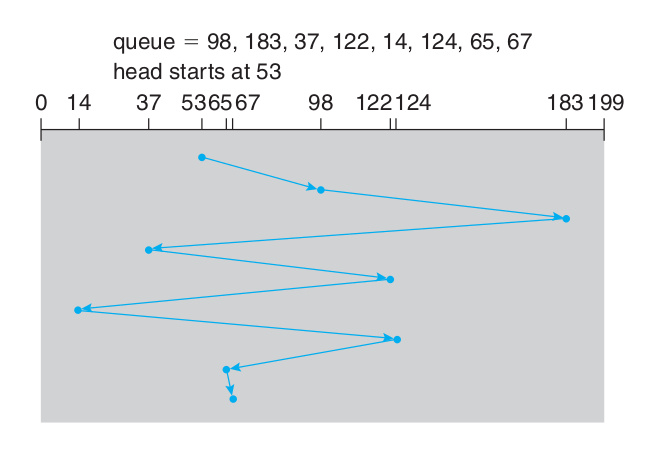
\includegraphics[width=0.7\textwidth]{imagenes/disco-fcfs}
	\caption{Recorrido del cabezal para algoritmo FCFS: El cabezal va desde el cilindro 53 hasta el 98, luego al 183, 37, 122, en orden hasta atender el último pedido en el cilindro 67. Se puede ver que si, en vez de haberlos hechos de esta manera, se hubiesen atendido primero el 37 y el 14 y después el 122 y el 124 también se hubiese reducido la distancia recorrida por el cabezal}
	\label{fig:disco-fcfs}
\end{figure}


\subsubsection{Shortest Seek Time First (SSTF)}
Se atienden primero los pedidos más cercanos al cabezal de escritura/lectura. 
Este algoritmo provee una sustancial mejora en el rendimiento del disco pero puede llegar a causar inanición de algunos pedidos, un escenario que se vuelve cada vez más probable a medida que la cola de espera crece.

\subsubsection{SCAN}
El brazo del disco comienza en un extremo del disco y se mueve hacia el final respondiendo pedidos a medida que va alcanzando cada cilindro. Una vez que termina de recorrer el disco, el brazo vuelve a repetir el proceso pero en la dirección inversa.

Si un pedido que esté justo enfrente del cabezal llega a la cola, entonces es resuelto inmediatamente. Si el cabezal ya pasó por ese sector, se deberá esperar a que el mismo llegue hasta el final del disco y vuelva hasta el sector correspondiente.

\subsection{Gestión del disco}
El sistema operativo también es responsable de manejar otros aspectos del disco:

\subsubsection{Formateo} 
Antes de porder guardar información en un disco, se lo debe dividir en sectores que el controlador del disco pueda leer y escribir. Este proceso es llamado \textbf{formateo de bajo nivel} o \textbf{formateo físico}. El formateo llena el disco con una estructura de datos especial para cada sector que consiste en un header, un área de datos y un \textit{posfijo}.

El header y el posfijo contienen información como el número del sectory codigo de corrección de errores. El controlador del disco actualiza esta información cada vez que realiza una escritura. Y la usa para comprobar que no haya fallas en ese sector cuando necesita leer del mismo. Si hay alguna falla, entonces puede usar el código de corrección de errores para recuperar la información corrupta. Sin embargo, esto solo es posible si solo fueron corrompidos uno pocos bits.

\subsubsection{Booteo} 
Cuando una computadora se enciende, necesita que se ejecute un programa llamado \textbf{bootstrap} que inicializa todos los aspectos del sistema (desde los registros de la CPU, los controladores de los dispositivos. el contenido de la memoria principal hasta el sistema operativo).

En la mayoria de las computadoras, se guarda un cargador de este programa (\textbf{bootsrap loader}) en una área de memoria de solo lectura (\textbf{read only memory - ROM}). El bootstrap loader se encarga de leer el programa de bootstrap desde disco. El mismo está ubicado en los bloques de inicialización (\textbf{boot blocks}) que están en una posición fija. 

\subsubsection{Bloques dañados}
Como los discos tienen partes movibles y tolerancias bajas, son propensos a fallas. En caso de que el fallo sea completo, el disco debe ser remplazado y no será posible recuperar su contenido a menos que se cuente con un disco de backup. 

En el caso de que solo haya sectores defectuosos, se pueden utilizar varias estrategias para manejarlos:
\begin{itemize}
	\item La más simple de todas, es escanear el disco para encontrar aquellos bloques defectuosos y marcarlos como inservibles para que el sistema operativo no los reserve.
	\item Otra técnica más sofisticada, es hacer que el controlador del disco mantenga una lista de los bloques defectuosos. Esta lista se inicializa durante el formateo de bajo nivel durante la fabriación y es actualizada constatemente durante la vida útil del disco.
	
	En este caso, el formateo genera sectores extra que no son visibles al sistema. De esta manera, cuando un bloque se daña, puede ser remplazado por uno de estos sectores sin mayores problemas.
\end{itemize}

\subsection{RAID}
Gracias a que los discos son cada vez mas baratos, es cada vez más factible tener varios discos en un sistema, lo que nos da la oportunidad de mejorar la velocidad de transferencia del sistema, y la seguridad de la información.

La solución para disminuir la probabilidad de perdida de datos, es agregar \textbf{redundancia}. Es decir, guardamos información que no es necesaria pero que puede usar en caso de que un disco falle para reconstruir la informción perdida.

La forma más simple (y más cara) de lograr esto es utilizar la técnica de \textbf{mirroring} que consiste en duplicar los datos de cada disco. En este caso, cada vez que se escribe algo a memoria, la operación se realiza en ambos discos por igual. Si algún disco falla, los datos pueden ser leídos del otro disco hasta que el disco dañado sea remplazado por uno nuevo.

Para mejorar la velocidad de transferencia se puede distribuir los bloques de un mismo archivo entre los discos. Está técnica es conocida como \textbf{\textit{data stripping}}. Cada disco participa en cada acceso a memoria 
lo que permite multiplicar la cantidad de información enviada por cada acceso de memoria.

Entonces \textbf{mirroring} provee alta seguridad de los datos pero es caro y \textbf{stripping} nos permite alcanzar altas velocidades de transferencia pero no mejora la seguridad. Por esta razón, se diseñaron varios esquemas que combinan estás dos técnicas de distintas maneras para lograr buenos trade-offs entre seguridad y ancho de banda.

Este conjunto de esquemas son conocidos como \textbf{Redundant Arrays of Independent Disks (RAID)} y están classificados en niveles:

\begin{itemize}
	\item \textbf{RAID 0 (Stripping):} Los bloques de un mismo archivo se distribuyen en dos (o más discos). No aporta ninguna redundancia, pero permite escrituras en paralelo lo que mejora el ancho de banda.
	\item \textbf{RAID 1 (Mirroring)}: Las escrituras se realizan en dos (o más) discos de manera simultanea. En el mejor de los casos tardan lo mismo que si tuviesemos un solo disco, en el peor tarda el doble. Mejora el rendimiento de las lecturas pero es demasiado caro de implementar.
	\item \textbf{RAID 2:} Tambien conocido como \textbf{memory-style error-correcting-code organizatio n(ECC)}. Se realiza un stripping a nivel bit de los datos que se guardan en discos distintos. Los códigos de corrección de error se guardan en discos aparte. Si un disco falla, entonces se puede usar el resto de los bits del archivo desde los otros discos y junto con su código de corrección correspondiente para recuperar la información perdida.
	\item \textbf{RAID 3:} Mejora el RAID 2 teniendo en cuenta que los controladores de disco pueden detectar si un sector fue leído correctamente por lo que un único bit de paridad puede ser usado tanto como para corregir como para detectar daños. Si uno de los sectores está dañado, sabemos que sector es y podemos calcular el valor del bit perdido a partir de la paridad de los sectores en los otros discos. Este tipo de RAID es igual de efectivo que el RAID 2 pero es más barato de implementar.
	
	Este nivel, es mejor que el nivel 1 porque se reduce la cantidad de discos necesarios para conseguir redundancia. Sin embargo, soporta menos operaciones de entrada/salida por segundo ya que todos los discos deben participar en cada transferencia. Además, puede llegar a ser muy caro computar la paridad de cada bloque.

	\item \textbf{RAID 4:} O \textbf{block-interleaved parity orgnaization} usa stripping a nivel de bloque, como raid 0, pero mantiene un disco a parte en el que se guarda bloques de paridad por cada bloque de los otros discos. Si un disco falla, se puede recuperar el bloque dañado usando los bloques del resto de los discos junto con el bloque de paridad.
	
	Un lectura accede solo un dico, por lo que es posible atender varios pedidos de manera simultanea por lo que el ancho de banda para lecturas es alto. Sin embargo, cuando se desean realizar escrituras de tamaños pequeños, es necesario cargar en memoria todo el bloque, modificarlo y luego volver a escribirlo en disco, además de actualizar el bloque de paridad. Esto puede alentizar el sistema.
	
	\item \textbf{RAID 5:} O \textbf{block-interleaved distributed parity} es el RAID 4 con la diferencia que los datos y los bloques de paridad se reparten entre todos los discos. Esto aligera la carga de los discos que hubiesen sido usados como discos de paridad, alargando su vida útil.
	
	\item \textbf{RAID 6:} Es como el RAID 5 pero almacena más información redudante para proteger de fallas de múltiples discos.
	
	\item \textbf{RAID 0 + 1:} Es una combinación de los RAID 0 y RAID 1. Se realiza un stripping de la data entre varios discos y luego se duplican esa escritura en otro conjunto de discos. Generalmente, tiene mejor performance que el RAID 5 pero duplica la cantidad de discos necesarios para implementarlo.
\end{itemize}

Por lo general, junto con estos esquemas se agrega un disco de respuesto que no es usado hasta que un disco falle completamente. Una vez que esto sucede, se reconstruye en el mismo la data perdida. Además RAID solo protege de errores físicos en los discos, no de errores  de otros hardware o software por lo que es necesario tener copias de seguridad y sistemas de archivos que brinden protección extra.

\printbibliography[keyword=discos, title=Bibliografía]

\newpage
\section{Sistemas de archivos}
El sistema de archivos (filesystem) es el módulo del kernel que se encarga de organizar la información de manera lógica. Es decir, se encarga de estructurar la información guardad en cada archivo y de como ordenarlos en su conjunto.

\subsection{Archivos}
Un archivo es un mecanismo de abstracción que provee una forma de guardar información en el disco. Nos permiten abstraer los detalles del método usado guardar la información deseada y como funciona el disco.

Cada archivo es identificado por un nombre que puede consistir en dos partes separadas por un punto. La segunda parte se conoce como la \textbf{extensión} del archivo y usualmente indica como está estructurado internamente. Sin embargo, el nombre (junto con la extensión) solo das a los usuarios una forma de distinguir fácilmente el tipo de contenido guardado en el mismo. Para el sistema operativo, el archivo es simplemente una secuencia de bytes sin sentido.

Esto nos da la máxima flexibilidad posible, ya que un usuario puede poner lo que quiera en sus archivos, de la forma que mejor le parezca. El sistema operativo no ofrece ninguna ayuda pero tampoco estorba.

Por lo general, los sistemas operativos soportan varios tipos de archivos. En los sistemas UNIX podemos distinguir los siguientes: 
\begin{itemize}
	\item Los \textbf{archivos regulares} son los archivos que contienen la información del usuario.
	\item Los archivos de \textbf{directorios} son los archivos que usa el sistema para mantener la estructura del filesystem.
	\item Los archivos de carácter especial (\textbf{character special files}) son usados para modelar dispositivos de entradas/salida como terminales, impresoras y redes.
	\item Los archivos especiales de bloques \textbf{Block Special Files} son usados para modelrar discos.
\end{itemize}

\subsubsection{Atributos}\label{atributos-archivos}
Cuando un usuario guarda un archivo, el filesystem, además de asociar el nombre con los datos correspondientes almacena varios atributos que le permitirán operar al sistema en el futuro. Estos atributos son conocidos como los \textbf{metadatos} del archivo y son almacenados en las estructuras de directorio.

Algunos ejemplos de metadatos son:
\begin{itemize}
	\item \textbf{Flags de protección:} Indican que operaciones podrá realizar cada usuario o grupo de usuarios sobre el archivo.
	\item \textbf{Tamaños}: El tamaño actual del achivo y, si está definido, el tamaño máximo permitido.
	\item \textbf{Propietario}: Un identificador del usuario que creó el archivo
	\item \textbf{Fechas de creación, modificación y acceso}
	\item\textbf{Bits de archivado}: Indica si hay alguna copia e seguridad del archivo.
	\item \textbf{Tipo de archivo}: Si es regular, directorio, representa algun dispositivo, etc.
	\item \textbf{Conteo de referencias}
	\item \textbf{CRC}
\end{itemize}

\subsection{Estructuras de directorios}
\paragraph{Volumen:} Una partición de un dispositivo, un dispositivo entero o un varios dispositivos que participan en un RAID que contienen un sistema de archivos. Cada volumen puede ser pensado como un disco virtual y es capaz de contener uno o más sistemas operativos. 

Cada volumen, además de contener un filesystem debe almacenar la información sobre los archivos que contiene el sistema. Una de las formas más simples de mantener esta información es en una tabla llamada  \textbf{directorio del dispositivo} o \textbf{tabla de contenidos del volumen}. La misma puede ser vista como una tabla que traduce nombres de archivos en sus entradas de directorio correspondientes (es decir, a punteros que indican donde están los metadatos del mismo).

Hoy en día, la mayoría de los sistemas operativos utiliza directorios estructurados en forma de árbol. Los mismos establecen una jerarquía de directorios que permiten al usuario crear sus propios subdirectorios y organizar sus archivos como mejor le parezca. 

\begin{figure}[h]
	\centering
	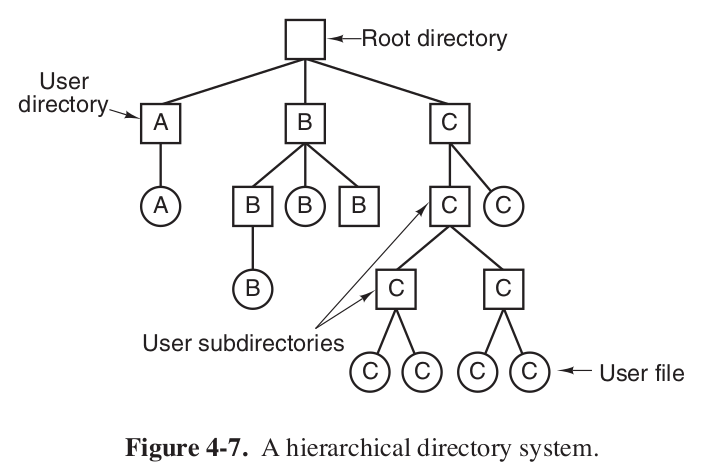
\includegraphics[width=0.7\textwidth]{imagenes/directorio-arbol}
	\label{fig:directorio-arbol}
\end{figure}


\subsubsection{Directorios de grafos áciclico (DAG)}
Consideremos dos porgramadores que están trabajando en el mismo projecto. Los archivos asociados con ese proyecto son guardados en un subidrectorio, separandolos así de otros projectos y archivos de cada uno de los programadores.

Un directorio con estructura de gráfo acíclico es una generalización a uso de un árbol que permite que se compartan archivos y directorios.

En este esquema, el mismo archivo o subdirectorio puede estar en dos directorios distintos de manera simultánea. Entonces se dice que ese archivo/subdirectorio es \textbf{compartido}. Es importante notar, que un archivo compartido no es lo mismo que tener dos copias del mismo archivo. Con dos copias, si un programador cambia su copia, el otro no verá los cambio en la suya. Con un archivo compartido, los cambios hechos por una persona son inmediatamente visibles por el otro.

En sistemas UNIX, este tipo los archivos y subdirectorios compartidos se crean agregando una nueva entrada de directorio al sistema llamado \textbf{link simbólico} que apunta al archivo o subdirectorio en cuestión.

Cuando se hace una referencia a un archivo, buscamos en el directorio. Si la entrada del directorio está marcada como link, entonces debemos resolverlo usando el nombre real del archivo al que apunta.

\begin{figure}[h]
	\centering
	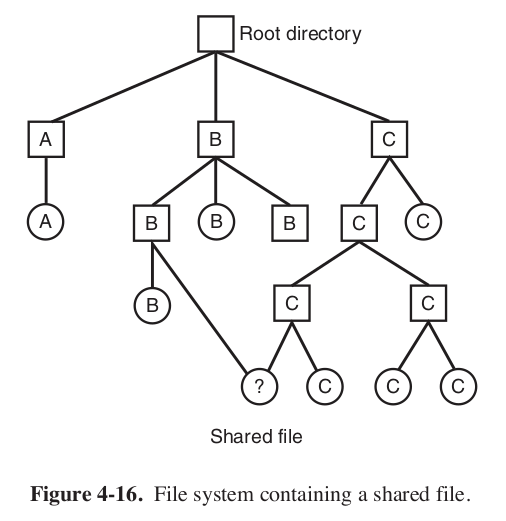
\includegraphics[width=0.6\textwidth]{imagenes/directorio-dag}
	\label{fig:directorio-dag}
\end{figure}

\subsection{Punto de montaje}
Así como hay que abrir un archivo antes de usarlo, un sistema de archivo debe ser \textbf{montado}. Mas específicamente, la estructura de directorio del sistema operativo se construye a partir de múltiples volumenes que deben ser montados para que estén disponibles al usuario.

El proceso de montaje es simple. Primero, se envia al sistema operativo el nombre del dispositivo y un \textbf{punto de montaje} (la ubicación dentro de la estructura de archivos a través de la cual el usuario podrá acceder al sistema de archivos). Algunos sistemas operativos tambien requieren el tipo de filesystem que va a ser montado, mientras que otros analizan la estructura del dispositivo para determinarlo. Por lo general, el punto de montaje es una directorio vacío.

Luego, el sistema operativo verifica que el dispositivo contiene un sistema de archivos válido y luego marca el punto de montaje como forma de acceso al mismo. Este esquema permite al usuario recorrer de manera uniforme diferentes sistemas de archivos.

\subsection{Representación de archivos}
El sistema de archivos maneja toda la metadata (atributos - ver \ref{atributos-archivos}) relacionada con los archivos y las estructuras de los directorios. Esta información está almacenada en bloques de control de archivos (file-control block).

\subsubsection{Representacion continua}
Una de las formas más fáciles de almacenar los archivos es guardandolos en bloques continuos en el disco. En este caso, los file-systems tienen que almacenar su file-control block la dirección del primer bloque y la cantidad de bloques ocupados por el archivo. Sin embargo, es un problema encontrar el espacio necesario para cada uno de ellos, es difícil saber cuanto espacio necesitara en el futuro atributos-archivos y produce fragmentación externa.

\subsubsection{Representacion como lista enlazada}
Soluciona todos los problemas de la representación continua. En este esquema, cada archivo es una lista enlazada de bloques de disco. El directorio contiene un puntero al primer y último bloque del archivo.

Para crear un archivo nuevo, simplemente creamos una entrada nueva en el directorio con sus punteros en \texttt{null}. Una escritura en el disco, hace que el sistema de manejo de memoria libre encuentre un bloque vacío.

Sin embargo, el mayor problema con esta representación es que el acceso aleatorio es ineficiente.

\begin{figure}[h]
	\centering
	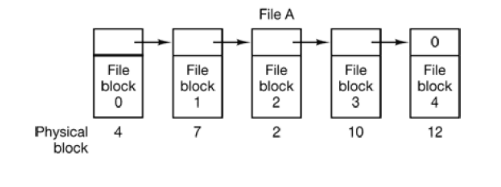
\includegraphics[width=0.6\textwidth]{imagenes/file-lista-enlazada}
	\caption{Archivo como lista enlazada}
	\label{fig:file-lista-enlazada}
\end{figure}

Una variación importante de este que esquema, es el uso de \textbf{file-allocation-table (FAT)}. En esta variación, se reserva una sección del disco para contener una tabla que indica, para cada bloque, cual es su siguiente y los bloques no usados son marcados con un símbolo especial. 

Entonces el problema de encontrar un bloque vacío se reduce a buscar en esta tabla el valor especial, sin embargo no es un esquema escalable ya que la misma puede llegar a ocupar mucho espacios y requerir varios movimientos de la cabeza del disco para leer un solo archivo (en el peor de los casos, un movimiento para leer la FAT y otro para leer el bloque por cada bloque del archivo).

\subsubsection{Indexación (inodos)}
Cada archivo tiene su propio bloque de indices. La $i$-ésima entrada en este bloque apunta al $i$-ésimo bloque del archivo. Cuando el archivo es creado, todos los punteros del bloque son inicializados en $null$ y se van modificando a medida que el archivo va creciendo.

Para permitir archivos que necesiten mas bloques que los que puede apuntar el bloque indice se pueden usar distintos esquemas:

\paragraph{Lista enlazada:} Los bloques de una archivo están definidos por una lista enlazada de bloques de índices.

\paragraph{Indice multinivel:} Se comienza con un bloque de indices cuyos punteros apuntan a un segundo bloque de índices que apuntan a los bloques del archivo.

\paragraph{Combinación de los ultimos dos:} Es lo que hace linux. Los file-control blocks (inodos), contienen los atributos, una lista de punteros que apuntan directamente a bloques del archivo (\textbf{direct blocks})(permiten acceder a archivos pequeños), luego un puntero a un bloque llamado \textbf{single indirect block} que apunta a una lista de \textbf{direct blocks}, luego otro puntero a un \textbf{double indirect block} y por último un puntero a un \textbf{triple indirect block}. Cada uno agregando un nivel más de indirección a los bloques del archivo

	\begin{figure}[h]
		\centering
		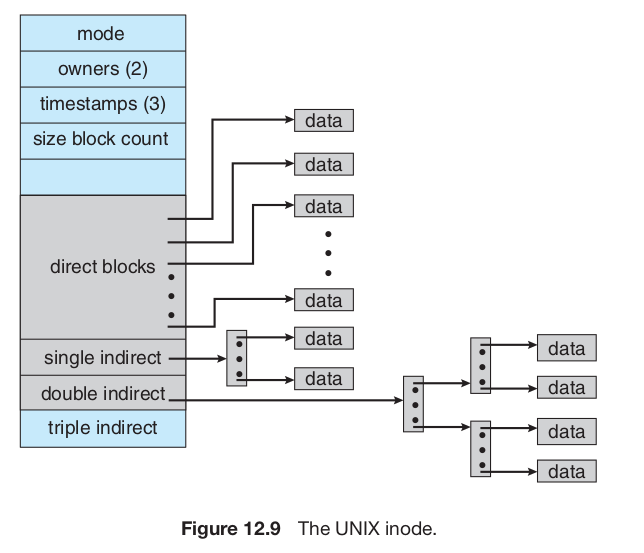
\includegraphics[width=0.5\textwidth]{imagenes/inodos}
		\caption{}
		\label{fig:inodos}
	\end{figure}

De esta manera solo es necesario mantener en memoria las tablas de los archivos abiertos (y solo las partes que se van usando de la misma).

En este caso, se reserva un inodo como entrada al directorio raíz y por cada archivo o subdirectorio hay una entrada que apunta a al inodo correspondiente.

\subsection{Manejo del espacio libre}
Dado que el espacio del disco es limitado y los archivos se van creando, modificando y borrando con el tiempo, el sistema mantiene una \textbf{lista de espacio libre} que indica cuales son los bloques libres del disco. De esta forma, para crear un archivo, se debe buscar en esta lista el espacio requerido. Luego, ese espacio se borra de dicha lista.

Hay varias formas de implementar esta lista:

\subsubsection{Bit Vector}
La forma más simple es usar un \textbf{bit map} o \textbf{vector bit}. Cada bloque esta representado por 1 bit. Si el bloque está libre, el bit es 1, si está siendo usado es un 0.

La principal ventaja de esta implementación es su relativa simplicidad y la eficiencia que tiene para encontrar el primer bloque libre en el disco. Sin embargo, son ineficientes salvo que se mantengantotalmente en memoria, lo cual es un problema si el disco es demasiado grande ya que puede llegar ocupar demasiado espacio.

\subsubsection{Listas enlazadas}
Otra forma es mantener un puntero al primer bloque libre del disco y cachearlo en memoria. El bloque contiene un puntero al siguiente bloque libre y así. Entonces la lista enlazada está repartida en los bloques libres del disco. Este esquema no eficiente: Para recorrer la lista debemos leer cada bloque lo que requiere un gran tiempo de I/O. Afortunadamente, esto no es algo que se haga usualemente. Por lo general, el sistema operativo, solo necesita un bloque libre para asignar un archivo. 

Se puede mejorar este método haciendo que cada bloque tenga $n$ punteros a bloques libres y un último puntero al siguiente bloque de la lista. De esta manera, se acelera el acceso a las direcciones de varios bloques.

Además, también se puede mantener punteros solo al primer bloque de una lista contigua de bloques y la cantidad de bloques contiguos. De esta manera, también nos ahorramos una cantidad gran cantidad de punteros.

\subsection{Perfomance}
Algunos sistemas separan una parte de la memoria principal para usarla como caché usando el sistema de paginación similar al visto en la sección \ref{paginacion}. Este tipo de caché trata la información de los archivos como páginas en vez de bloques, esto nos permite unificar los accesos de los procesos con la memoria virtual en vez de utilizar el sitema de archivos: Este esquema se llama \textbf{memoria virtual unificada}.

Otro problema que puede afectar la perfomance del sistema es si las operaciones  de I/O son síncronas o asíncronas. Las \textbf{ escrituras síncronas} ocurren en el el orden en el que el subsistema de disco recibe los pedidos y las escrituras no se bufferean. En las \textbf{escrituras asíncroncas}, los datos son almacenados en la caché y se devuelve el control al proceso. Luego la caché es bajada a memoria en otro momento. Por lo general, las escrituras se hacen de manera asincroca, sin embargo los sistemas operativos incluyen un flag en la system \texttt{open} que permiten a un proceso requerir escrituras sincrónicas.

\subsection{Recuperación}
Los archivos y directorios deben ser mantenidos tanto en memoria principal como en disco y se debe asegurar que una falla en sistema no resulte en perdida de información o incosistencia en las estructuras de datos del filesystem.

\subsubsection{Consistencia}
Cualquiera sea la causa de corrupción, un sistema de archivos debe detectar el problema y corregirlo. Para detectarlo, se puede escanear la metadata de cada archivo para confirmar su estado. Sin embargo, esto puede llegar a tomar varias horas si el sistema es muy grande y debería hacerse cada vez que el sistema bootea.

Alternativamente, el sistema de archivos puede almacenar su estado en la meta-data del sistema:  Un bit se setea cuando se están produciendo cambios en los datos del sistema. Si todas las actualizaciones son completadas correctamente, entonces se limpia el bit. Si esto no sucede, se debe correr un programa llamado \textbf{consistency checker} que realiza el escaneo mencionado y trata de corregir las inconsistencias que encuentre.

\subsubsection{Journaling}
Con el verificador de incosistencias, permitimos que las estucturas se rompan y las reparamos en la fase de recuperación. Sim embargo, este método tiene varios problemas: Puede haber inconsistencias irreparables, puede requerir intervención humana y tomar mucho tiempo.

La solución a este problema es aplicar técnicas de recuperación basadas en logging: Cada conjunto de operaciones para realizar una tarea específica en el disco es llamada \textbf{transacción}. Primero se escriben en un log todos los cambios, se consideran como listos para \textit{commitear} (escribir en disco) y se devuelve el control al proceso. Mientras tanto, las entradas escritas en el log se ejecutan en el sistema de archivos.

A medida que estas acciones se van completando, se actualiza un puntero que indica cual es la próxima acción a realizar. Una vez que se terminó de commitear una transacción, la misma se remueve del log (que suele ser un \textbf{buffer circular}).

Si el sistema falla, el log tendrá cero o más transacciones que no fueron completadas, por lo que deben terminarse. El sistema puede retomar la ejecución desde el puntero guardado y se puede recuperar la consistencia del sistema. Si la transacción fue abortada, entonces sus cambios deben revertirse. 

Este registro se escrbie en bloques consecutivos, por lo que para modificarlo, se realiza una escritura secuencial y el impacto en performance es bajo.

\subsection{Network File System}
Con la evolución de la red y la tecnología de archivos, los métodos de compartir archivos han cambiado. Los primeros métodos implementados consistian en transferir manualmente los archivos usando programos como \textbf{ftp}. Luego, se comenzaron a usar sistemas de archivos distribuidos (distributed file system - DFS) en la cual los directorios remotos son visibles desde una computadora local. El tercer: \textbf{World Wide Web} es, en cierto modo es una reversión al primer método, ya que es necesario un navegador web para poder acceder a los archivos remotos y distintas operaciones son usadas para transferir archivos.

Los sistemas de archivos de red son protocolos que permiten acceder a sistemas de archivos remotos como si fuesen locales usando llamadas a procedimientos remotos. Para esto se define un protocolo de montaje que permite montar el file system remoto en el sistema local como si  fuese una parte integral del de sistema de archivos locales. Para poder soportar esto, los SO implementan una capa llamada \textbf{Virtual File System} que contiene \textit{vnodes} por cada archivo abierto. Así, los pedidos de E/S que llegan a este sistema son despachados al sistema de archivos locales o al sistema de archivos de red de manera transparente.

Si bien es necesario un módulo de kernel especial del lado del cliente, del lado del server alcanza con un programa común y corriente.
\printbibliography[keyword=filesystem, title=Bibliografía]

\newpage
\section{\red{Sistemas de archivos}}
	\subsection{\red{Responsabilidades del FS}}
	% TODO
	\subsection{\red{Punto de montaje}}
	% TODO
	\subsection{\red{Representación de archivos}}
	% TODO
	\subsection{\red{Manejo del espacio libre}}
	% TODO
	\subsection{\red{FAT, inodos}}
	% TODO
	\subsection{\red{Atributos}}
	% TODO
	\subsection{\red{Directorios}}
	% TODO
	\subsection{\red{Caché}}
	% TODO
	\subsection{\red{Consistencia, journaling}}
	% TODO
	\subsection{\red{Características avanzadas}}
	% TODO
	\subsection{\red{NFS, VFS}}
	% TODO


\newpage
\section{\red{Protección y seguridad}}
	\subsection{\red{Conceptos de protección y seguridad}}
	% TODO
	\subsection{\red{Matrices de permisos}}
	% TODO
	\subsection{\red{MAC vs. DAC}}
	% TODO
	\subsection{\red{Autenticación, autorización y auditoría}}
	% TODO
	\subsection{\red{Funciones de hash de una vía}}
	% TODO
	\subsection{\red{Encriptación simétrica}}
	% TODO
	\subsection{\red{RSA}}
	% TODO
	\subsection{\red{Privilegios de procesos}}
	% TODO
	\subsection{\red{Buffer overflows}}
	% TODO
	\subsection{\red{Inyección de parámetros}}
	% TODO
	\subsection{\red{Condiciones de carrera}}
	% TODO
	\subsection{\red{Sandboxes}}
	% TODO
	\subsection{\red{Principios generale de seguridad}}
	% TODO



\newpage
\part{\red{Conceptos avanzados}}
\section{\red{Sistemas distribuidos}}
\subsection{\red{Taxonomía de Flynn}}
% TODO
\subsection{\red{Arquitecturas de HW y SW para sistemas distribuidos}}
% TODO
\subsection{\red{RPC}}
% TODO
\subsection{\red{Threads}}
% TODO
\subsection{\red{Pasaje de mensajes}}
% TODO
\subsection{\red{Orden parcial entre eventos}}
% TODO
\subsection{\red{Livelock}}
% TODO
\subsection{\red{Acuerdo bizantino}}
% TODO
\subsection{\red{Intuición de safety, liveness, fairness}}
% TODO
\subsection{\red{Algoritmo del banquero}}
% TODO
\subsection{\red{Panadería de Lamport}}
% TODO
\subsection{\red{Modelos de fallas y métricas de complejidad}}

% TODO
\subsection{\red{Exclusión mutua y locks distribuidos}}
% TODO
\subsection{\red{Elección de líder}}
% TODO
\subsection{\red{Instantánea global consistente}}
% TODO
\subsection{\red{2PC}}
% TODO

	\section{\red{Virtualización}}
	% TODO
	\section{\red{Contenedores}}
	% TODO
	\section{\red{Cloud computing}}
	% TODO

	
\end{document}

